\documentclass[a4paper, 12pt]{extarticle}

\usepackage{xecyr}
\usepackage{color}
\usepackage{float}
\usepackage{fontenc}
\usepackage{amsmath}
\usepackage{xltxtra}
\usepackage{graphicx}
\usepackage{csquotes}
\usepackage{listings}
\usepackage{longtable}
\usepackage{indentfirst}
\usepackage[russian]{babel}

\usepackage{amssymb}
% \usepackage{cite}
\usepackage{doi}
\usepackage{subfig}
\usepackage[labelfont=bf,labelsep=period]{caption}

\usepackage{titlesec}
\titleformat{\section}
  {\normalfont\fontsize{14}{15}\bfseries}{\thesection.}{5pt}{}
\titleformat{\subsection}
  {\normalfont\fontsize{14}{15}\bfseries}{\thesubsection.}{5pt}{}
\titleformat{\subsubsection}
  {\normalfont\fontsize{14}{15}\bfseries}{\thesubsubsection.}{5pt}{}

\usepackage{fontspec}
\defaultfontfeatures{Ligatures=TeX}
\setmainfont[Ligatures=TeX]{Times New Roman}

\usepackage[a4paper,margin=1in,heightrounded]{geometry}
\geometry{left=1.5cm}
\geometry{right=1.5cm}
\geometry{top=2cm}
\geometry{bottom=2cm}

\usepackage{expl3}
\ExplSyntaxOn
\cs_new_eq:NN \Repeat \prg_replicate:nn
\ExplSyntaxOff

\usepackage[maxnames=5,
        backend=biber,
        style=gost-numeric,
        sorting=none,
        autolang=other]{biblatex}
\addbibresource{bibliography.bib}

% Sections style redefinition
\renewcommand{\thesection}
  {\thepart\arabic{section}}
\renewcommand{\thesubsection}
  {\thepart\arabic{section}.\arabic{subsection}}
\renewcommand{\thesubsubsection}
  {\thepart\arabic{section}.\arabic{subsection}.\arabic{subsubsection}}


% Equations, fugures, tables numbering style redefinition
\renewcommand{\theequation}
  {\arabic{equation}}
\renewcommand{\thefigure}
  {\arabic{figure}}
\renewcommand{\thetable}
  {\arabic{table}}

% Enum style redefinition
\renewcommand{\labelenumii}
  {\labelenumi\arabic{enumii}.}
\renewcommand{\labelenumiii}
  {\labelenumii\arabic{enumiii}.}

% Enlarge table row height
\renewcommand{\arraystretch}{1.2}

% Font to inline code highlighting
% Consolas must be installed!!!
\newfontfamily{\codefont}[Scale=0.9]{Consolas}
\newfontfamily{\listingsfont}[Scale=1.0]{Consolas}

% Define default style for codelisitngs
\definecolor{codegreen}{rgb}{0.00, 0.50, 0.00}
\definecolor{codegray} {rgb}{0.50, 0.50, 0.50}
\definecolor{codenumb} {rgb}{0.00, 0.00, 1.00}
\definecolor{codeblue} {rgb}{0.00, 0.43, 0.13}
\definecolor{codebrick}{rgb}{0.64, 0.08, 0.08}
\lstset{
  backgroundcolor=\color{white},
  basicstyle=\fontsize{10}{12}\selectfont\listingsfont,
  breakatwhitespace=false,
  breaklines=true,
  captionpos=b,
  commentstyle=\color{codegreen},
  frame=l,
  keepspaces=true,
  keywordstyle=\color{codeblue},
  language=C++,
  numbers=left,
  numbersep=8pt,
  numberstyle=\tiny\color{codegray},
  rulecolor=\color{black},
  showspaces=false,
  showstringspaces=false,
  showtabs=false,
  stepnumber=1,
  stringstyle=\color{codebrick},
  tabsize=2,
  title=\lstname
}

% Listing numbering style redefinition
\renewcommand{\lstlistingname}{Листинг}
\AtBeginDocument{
  \renewcommand{\thelstlisting}{\thesection\arabic{lstlisting}}
}

\newtheorem{hypothesis}{Гепотеза}
\newtheorem{theorem}{Теорема}

\DeclareMathOperator*{\argmax}{arg\,max}
\DeclareMathOperator*{\argmin}{arg\,min}
\DeclareMathOperator{\sign}{sign}
\DeclareMathOperator{\re}{\operatorname{Re}}

\begin{document}

\begingroup
\fontsize{14pt}{17pt}\selectfont
\begin{titlepage}

  \begin{center}
    \fontsize{14pt}{0pt}

    Федеральное государственное автономное образовательное учреждение \\*
    высшего образования «Национальный исследовательский \\*
    Нижегородский государственный университет им. Н.И. Лобачевского»\\
  \end{center}

  \vspace{12pt}
  \vspace{25pt}

  \begin{center}
  \fontsize{14pt}{0pt}
  \textit{На правах рукописи\\}

  \vspace{12pt}

  CОВРАСОВ ВЛАДИСЛАВ ВАЛЕРЬЕВИЧ\\*
  \vspace{12pt}
  \vspace{25pt}
  \textbf{Разработка и исследование способов распределения ресурсов в\\*
  параллельных алгоритмах глобальной оптимизации}\\*
  \vspace{14pt}
  Направление подготовки\\*
  09.06.01 – Информатика и вычислительная\\*
  техника\\*
  \vspace{14pt}
  Направленность подготовки\\*
  05.13.18 – Математическое моделирование,\\*
  численные методы и комплексы программ\\*
  \vspace{14pt}
  \vspace{14pt}
  \textbf{Научный доклад об основных результатах\\*
  научно-квалификационной работы (диссертации)}
  \end{center}

  \vspace{40pt}


  \begin{flushright}
  Научный руководитель:\\
  д. т. н., доцент,\\
  Баркалов К. А.\\
  \end{flushright}

  \vspace{30pt}

  \vspace{\fill}

  \begin{center}
  Нижний Новгород \\*
  2021
  \end{center}

  \end{titlepage}
 % Link to main page
\endgroup

\begingroup
\fontsize{12pt}{20pt}\selectfont

\newpage
\thispagestyle{empty}
\tableofcontents

\newpage
\setcounter{page}{1}
\cs{Введение}

\subsection*{Актуальность темы исследования}

Задачи нелинейной глобальной оптимизации встречаются в различных прикладных областях (например, поиск оптимального
управление или гиперпараметров метода машинного обучения),
и традиционно считаются одними из самых трудоёмких среди оптимизационных задач.
Их сложность экспоненциально растёт в зависимости от размерности пространства поиска.
Зачастую глобальная оптимизация при размерности пространства в 10 переменных сложнее,
чем локальная оптимизация в существенно многомерном пространстве.
Для последней может оказаться достаточно применения простейшего метода градиентного спуска
или эвристических алгоритмов поиска по шаблону,
в то время как чтобы \textit{гарантированно} отыскать глобальный оптимум, методам
оптимизации приходится накапливать информацию о поведении целевой функции во всей области поиска.

На практике в роли параметров для оптимизации могут выступать параметры математической модели, например, при решении
задачи поиска оптимального управления или при настройке алгоритма машинного обучения под конкретные данные.
В этих случаях о поведении целевой функции (выпуклость, наличие производных) ничего неизвестно, т.е. метод оптимизации
работает с функцией, представляющей собой чёрный ящик. Кроме того, подобный чёрный ящик, как правило,
имеет высокую вычислительную сложность, во много раз превосходящую вычислительную сложность решающих правил метода оптимизации.

Широко представленным классом методов, решающих задачи с трудоёмкой целевой функцией типа чёрный ящик, являются
алгоритмы липшицевой глобальной оптимизации. Они требуют, чтобы целевая функция удовлетворяла условию Липшица в области поиска,
что является более сильным свойством, чем непрерывность, но более слабым, чем предположение о наличии непрерывных частных производных.
В то же время, этого достаточно, чтобы гарантировать глобальную сходимость при условии выбора
подходящих параметров применяемого метода оптимизации.

В задачах глобальной оптимизации область допустимых значений целевой функции также может быть определена
с помощью условий, например в виде функциональных ограничений типа неравенство. Это вносит дополнительную сложность в процесс решения
задач, требуя создания схем учёта ограничений. Ещё более сложными являются задачи многокритериальной условной многокритериальной
оптимизации и смешанного программирования. В последнем случае как целевая функция, так и функциональные ограничения
зависят и от непрерывных, и от дискретных переменных. Существуют методы скаляризации многокритериальных задач.
При этом порождается множество скалярных задач, каждую из которых необходимо решить. Задачи смешанного программирования
в некоторых случаях тоже можно свести к серии задач, каждая из которых соответствует одному дискретному параметру.
Решение серии задач условной глобальной задач при ограниченных вычислительных
ресурсах налагает дополнительные требования на метод оптимизации: помимо поиска глобального экстремума необходимо
распределять вычислительные ресурсы так, чтобы сразу во всех решаемых задачах положение глобального
экстремума было оценено примерно с одинаковым качеством.

Многообразие постановок задач и методов их решения говорит о том, что глобальная оптимизация
является развивающимся и актуальным направлением исследований в теории оптимизации, широко применяемым на практике.

\subsection*{Цель квалификационной работы}

Целью квалификационной работы является исследование и разработка последовательных и параллельных алгоритмов для
решения задач глобальной оптимизации, в частности разработка метода, который бы эффективно распределял ресурсы между задачами при
решении множества задач условной оптимизации.

Для достижения поставленной цели, необходимо решить следующие задачи:
\begin{enumerate}
    \item Сделать обзор современных методов глобальной оптимизации;
    \item Сравнить актуальные методы между собой;
    \item Сформулировать собственную модификацию алгоритма, решающего множество задач условной глобальной оптимизации,
    получить условия сходимости;
    \item Оценить качество работы полученного метода на большом наборе разнообразных тестовых задач с ограничениями.
\end{enumerate}

\textbf{Объект исследования} -- программные системы для решения задач глобальной оптимизации в различных постановках.

\textbf{Предмет исследования} -- методы решения задач условной глобальной оптимизации, теория их сходимости.

\subsection*{Обоснование специальности}

Область исследования соответствует следующим пунктам паспорта специальности 05.13.18 --
«Математическое моделирование, численные методы и комплексы программ»:
4. Реализация эффективных численных методов и алгоритмов в виде
комплексов проблемно-ориентированных программ для проведения
вычислительного эксперимента; 3. Разработка, обоснование и тестирование эффективных вычислительных
методов с применением современных компьютерных технологий.

\subsection*{Научная новизна}

В процессе работы была, разработана модификация метода для решения множества задач условной оптимизации, поддерживающая
функциональные ограничения типа неравенство.
Новизна работы заключается в следующем:

\begin{enumerate}
    \item Предложена модификация алгоритма AGS, которая менее чувствительна к параметрам и сходится так же быстро, как AGS
    с заранее подобранными под класс задач параметрами;
    \item Реализована поддержка нелинейных ограничений в алгоритме, решающeм
    множество задач глобальной оптимизации в совокупности и распределяющего свои ресурсы так, чтобы
    обеспечивать равномерную сходимость во всех задачах. Доказано теорема о достаточных условиях сходимости
    полученного метода. Свойство равномерной сходимости проверено с помощью численного эксперимента.
\end{enumerate}

\subsection*{Обоснованность и достоверность результатов}
Достоверность результатов, полученных в ходе выполнения квалификационной работы, подтверждается
тем, что различные части работы были опубликованы в рецензируемых сборниках трудов российских и международных конференций.
Кроме того, программная реализация метода AGS-AR прошла процедуру ревью и была включена в состав популярной библиотеки
алгоритмов нелинейной оптимизации NLOpt.

\textbf{Публикации.} Основные результаты по теме квалификационной работы изложены в трёх публикациях \cite{barkalovSovraov2019,sovrasov2019,sovrasov2020},
каждая из которых входит в сборник трудов конференций, индексируемый в базе данных Scopus.

\subsection*{Структура и объемы работы}

Квалификационная работа включает в себя введение, три главы, заключение и список литературы.
Полный объём квалификационной работы составляет 38 страниц, включая 11 рисунков и 6 таблиц.
Список литературы содержит 49 позиций.

\subsection*{Личный вклад автора}

Личный вклад автора состоит в следующем:

\begin{enumerate}
    \item Разработка методов, теоретический анализ их сходимости, их программная реализация.
    \item Разработка плана вычислительных экспериментов, их проведение, анализ результатов.
    \item Подготовка публикаций по проделанной работе.
\end{enumerate}

\section{Постановки задачи глобальной оптимизации, обзор существующих методов решения}


\subsection{Задача глобальной оптимизации с функциональными ограничениями-неравенствами}
В рамках данной работы будем рассматривать следующую постановку задачи глобальной
оптимизации: найти глобальный минимум \(N\)-мерной функции \(\varphi(y)\) в гиперинтервале
\(D=\{y\in \mathbf{R}^N:a_i\leqslant x_i\leqslant{b_i}, 1\leqslant{i}\leqslant{N}\}\).
Для построения оценки глобального минимума по конечному количеству вычислений
значения функции требуется, чтобы скорость изменения \(\varphi(y)\) в \(D\) была ограничена.
В качестве такого ограничения как правило принимается условие Липшица.
\begin{equation}
\label{eq:task}
\varphi(y^*)=\min\{\varphi(y):y\in D\}
\end{equation}

\begin{equation}
\label{eq:lip}
|\varphi(y_1)-\varphi(y_2)|\leqslant L\Vert y_1-y_2\Vert,y_1,y_2\in D,0<L<\infty
\end{equation}

Существуют различные методы, решающие рассмотренную многомерную задачу напрямую \cite{SergeyevKvasov2017, Jones2009},
а также эффективные методы решения одномерных задач \cite{Norkin1992, Strongin2000}. В данной работе рассматривается одномерный метод,
который применяется совместно со схемой редукции размерности.
Классической схемой редукции размерности исходной задачи для алгоритмов глобальной оптимизации является
использование разверток --- кривых, заполняющих пространство \cite{Sergeyev2013}.
\begin{equation}
\label{cube}
\lbrace y\in \mathbf{R}^N:-2^{-1}\leqslant y_i\leqslant 2^{-1},1\leqslant i\leqslant N\rbrace=\{y(x):0\leqslant x\leqslant 1\}
\end{equation}

Отображение вида (\ref{cube}) позволяет свести задачу в многомерном пространстве к решению
одномерной ценой ухудшения ее свойств. В частности, одномерная функция \(\varphi(y(x))\)
является не Липшицевой, а Гёльдеровой:
\begin{displaymath}
\label{holder}
|\varphi(y(x_1))-\varphi(y(x_2))|\leqslant H{|x_1-x_2|}^{\frac{1}{N}},x_1,x_2\in[0;1],
\end{displaymath}
где константа Гельдера \(H\) связана с константой Липшица \(L\) соотношением
\begin{equation}
  \label{eq:conv_cond}
 %H=4Ld\sqrt{N},d=\max\{b_i-a_i:1\leqslant i\leqslant N\}.
 H\leqslant 2L\sqrt{N+3}
\end{equation}

Область \(D\) также может быть задана с помощью функциональных ограничений, что
значительно усложняет задачу.
Постановка задачи глобальной оптимизации в этом случае будет иметь следующий вид:
\begin{equation}
  \label{eq:constrained_problem}
  \varphi(y^*)=\min\{\varphi(y):g_j(y)\leqslant 0, 1\leqslant j\leqslant m\}
\end{equation}
Обозначим \(g_{m+1}(y)=\varphi(y)\). Далее будем предполагать, что все функции \(g_k(y),1\leqslant k \leqslant m+1\)
удовлетворяют условию Липшица в некотором гиперинтервале, включающем \(D\).

\subsection{Серия задач глобальной оптимизации}

Также будем интересоваться решением серии из \(q\) задач вида (\ref{eq:constrained_problem}):
\begin{equation}
  \label{eq:many_problems}
  \min\left\{\varphi_1(y), y\in D_1 \right\}, \min\left\{\varphi_2(y), y\in D_2\right\},..., \min\left\{\varphi_q(y), y\in D_q\right\}.
\end{equation}

При решении серии задач (\ref{eq:many_problems}) возникает проблема оптимального распределения ресурсов метода между ними.
Будем считать, что метод оптимально распоряжается ресурсами, если при его остановке на некоторой итерации
решение всех задач получено с одинаковой точностью. Такого совйства можно добиться, потребовав
от метода равномерной сходимости на всём множестве задач:
\begin{equation}
  \label{eq:uni_conv}
  \exists \varepsilon > 0: \forall s>1, \forall i,j\in\{1,\dots,q\}\;
    \frac{\Vert \tilde{y_i}(s)^* - y_i*\Vert_\infty}{\Vert \tilde{y_j}(s)^* - y^*_j\Vert_	\infty} \leqslant \varepsilon,
\end{equation}
где \(s\) это количество итераций метода оптимизации, \(\tilde{y_i}(s)^*\) это приближение к решению, полученное методом в задаче \(i\)
из множества (\ref{eq:many_problems}) на итерации \(s\).

\subsection{Различные подходы к решению задач глобальной оптимизации}

\subsubsection{Стохастические методы}


\subsubsection{Детерминированные методы}


\paragraph{Индексный алгоритм глобального поиска}
В качестве римера детерминированного характеристического метода приведём индексный алгоритм глобального поиска \cite{Strongin2000}.

Принимая во внимание схему редукции размерности (\ref{cube}), будем при описании метода считать, что
требуется найти глобальный минимум функции \(\varphi(x), x\in[0;1]\),
удовлетворяющей условию Гёльдера, при ограничениях \(g_j(x)\), также
удовлетворяющих этому условию на интервале \([0;1]\).

Рассматриваемый индексный алгоритм глобального поиска (IAGS) для решения
одномерной задачи (\ref{eq:constrained_problem}) предполагает построение последовательности
точек \(x_k\), в которых вычисляются значения минимизируемой функции или ограничений \(z_k = g_s(x_k)\).
Для учета последних используется индексная схема \cite{Strongin2000}. Пусть \(Q_0=[0;1]\). Ограничение, имеющее номер
 \(j\), выполняется во всех точках области
\begin{displaymath}
  Q_j=\left\{x\in [0;1]:g_j(x)\leq 0\right\},
\end{displaymath}
которая называется допустимой для этого ограничения. При этом допустимая область \(D\)
исходной задачи определяется равенством: \(D=\cap _{j=0}^{m}Q_{j}\).
Испытание в точке \(x\in [0;1]\) состоит в последовательном вычислении значений
величин \(g_{1}(x),...,g_{\nu }(x)\), где значение индекса \(\nu\) определяется условиями:
\(x\in Q_{j},0\leqslant j<\nu ,x\notin Q_{\nu }\). Выявление первого нарушенного ограничения
прерывает испытание в точке \(x\). В случае, когда точка \(x\)  допустима, т. е.
\(x\in D\) испытание включает в себя вычисление всех функций задачи. При этом значение
индекса принимается равным величине \(\nu =m+1\). Пара \(\nu =\nu (x),z=g_{\nu }(x)\),
где индекс \(\nu\) лежит в границах \(1\leqslant \nu \leqslant m+1\), называется результатом
испытания в точке \(x\).

Такой подход к проведению испытаний позволяет свести исходную задачу с функциональными
ограничениями к безусловной задаче минимизации разрывной функции:

\begin{displaymath}
  \begin{array}{lr}
    \psi (x^{*})=\min_{x\in [0;1]}\psi (x), \\
    \psi (x)={\begin{cases}g_{\nu }(x)/H_{\nu }&\nu <M\\(g_{M}(x)-g_{M}^{*})/H_{M}&\nu =M\end{cases}}
  \end{array}
\end{displaymath}

Здесь \(M=\max_{}^{}\left\{\nu (x):x\in [0;1]\right\}\), а \(g_{M}^{*}=\min _{}^{}\left\{g_{M}(x):x\in \cap _{i=0}^{M-1}Q_{i}\right\}\).
В силу определения числа \(M\), задача отыскания \(g_{M}^{*}\)
всегда имеет решение, а если \(M=m+1\), то \(g_{M}^{*}=\varphi(x^{*})\).
Дуги функции \(\psi (x)\) гельдеровы на множествах \(\cap _{i=0}^{j}Q_{i},0\leq j\leq M-1\)
с константой 1, а сама \(\psi (x)\) может иметь разрывы первого рода на границах этих множеств.
Несмотря на то, что значения констант Гёльдера \(H_k\) и величина \(g_{M}^{*}\) заранее неизвестны,
они могут быть оценены в процессе решения задачи.

Множество троек \(\{(x_k,\nu_k,z_k)\}, 1\leqslant k\leqslant n\) составляет поисковую информацию,
накопленную методом после проведения \(n\) шагов.

На первой итерации метода испытание проводится в произвольной внутренней точке \(x_1\)
интервала \([0;1]\). Индексы точек 0 и 1 считаются нулевыми, значения \(z\) в
них не определены. Пусть выполнено \(k\geqslant 1\) итераций метода,
в процессе которых были проведены испытания в \(k\) точках \(x_i, 1\leqslant i\leqslant k\).
Тогда точка \(x^{k+1}\) поисковых испытаний следующей \((k+1)\)-ой
итерации определяются в соответствии с правилами:

Шаг 1. Перенумеровать точки множества \(X_k=\{x^1,\dotsc,x^k\}\cup\{0\}\cup\{1\}\),
которое включает в себя граничные точки интервала \([0;1]\), а также точки предшествующих
испытаний, нижними индексами в порядке увеличения значений координаты, т.е.
\begin{equation}
  \label{eq:points}
0=x_0<x_1<\dotsc<x_{k+1}=1
\end{equation}
и сопоставить им значения \(z_{i}=g_{\nu }(x_{i}),\nu =\nu (x_{i}),i={\overline {1,k}}\).

Шаг 2. Для каждого целого числа \(\nu ,1\leqslant \nu \leqslant m+1\) определить соответствующее
ему множество \(I_{\nu }\) нижних индексов точек, в которых вычислялись значения
функций \(g_{\nu }(x)\):
\begin{displaymath}
  I_{\nu }=\{i:\nu (x_{i})=\nu ,1\leqslant i\leqslant k\},1\leq \nu \leqslant m+1,
\end{displaymath}
определить максимальное значение индекса \(M=\max\{\nu (x_{i}),1\leq i\leq k\}\).

Шаг 3. Вычислить текущие оценки для неизвестных констант Гёльдера:
\begin{equation}
  \label{eq:step2}
  \mu _{\nu }=\max\{\frac{|g_{\nu }(x_{i})-g_{\nu }(x_{j})|}{(x_{i}-x_{j})^{\frac{1}{N}}}:i,j\in I_{\nu },i>j\}.
\end{equation}
Если множество \(I_{\nu }\) содержит менее двух элементов или если значение \(\mu _{\nu }\)
оказывается равным нулю, то принять \(\mu _{\nu }=1\).

Шаг 4. Для всех непустых множеств \(I_{\nu },\nu ={\overline {1,M}}\) вычислить оценки
\begin{equation}
  \label{eq:step_4}
  z_{\nu }^{*}={\begin{cases}\min\{g_{\nu }(x_{i}):x_{i}\in I_{\nu }\}&\nu =M\\-\varepsilon _{\nu }&\nu <M\end{cases}},
\end{equation}
где вектор с неотрицательными координатами \(\varepsilon _{R}=(\varepsilon _{1},..,\varepsilon _{m})\) называется вектором резервов.

Шаг 5. Для каждого интервала \((x_{i-1};x_{i}),1\leqslant i\leqslant k\) вычислить характеристику
\begin{equation}
  \label{eq:step3_1}
  R(i)={\begin{cases}\Delta _{i}+{\frac {(z_{i}-z_{i-1})^{2}}{(r_{\nu }\mu _{\nu })^{2}\Delta _{i}}}-2{\frac {z_{i}+z_{i-1}-2z_{\nu }^{*}}{r_{\nu }\mu _{\nu }}}&\nu =\nu (x_{i})=\nu (x_{i-1})\\2\Delta _{i}-4{\frac {z_{i-1}-z_{\nu }^{*}}{r_{\nu }\mu _{\nu }}}&\nu =\nu (x_{i-1})>\nu (x_{i})\\2\Delta _{i}-4{\frac {z_{i}-z_{\nu }^{*}}{r_{\nu }\mu _{\nu }}}&\nu =\nu (x_{i})>\nu (x_{i-1})\end{cases}}
\end{equation}
где \(\Delta _{i}=(x_{i}-x_{i-1})^{\frac{1}{N}}\). Величины \(r_{\nu }>1,\nu ={\overline {1,m}}\)
являются параметрами алгоритма. От них зависят произведения \(r_{\nu }\mu _{\nu }\),
используемые при вычислении характеристик в качестве оценок неизвестных констант Гёльдера.

Шаг 6. Выбрать наибольшую характеристику:
\begin{equation}
\label{step4}
t=\argmax_{1\leqslant i \leqslant k+1}R(i)
\end{equation}

Шаг 7. Провести очередное испытание в середине интервала \((x_{t-1};x_{t})\),
если индексы его концевых точек не совпадают: \(x^{k+1}={\frac {1}{2}}(x_{t}+x_{t-1})\).
В противном случае провести испытание в точке
\begin{displaymath}
  x^{k+1}={\frac {1}{2}}(x_{t}+x_{t-1})-\operatorname {sgn}(z_{t}-z_{t-1}){\frac {|z_{t}-z_{t-1}|^{n}}{2r_{\nu }\mu _{\nu }^{n}}},\nu =\nu (x_{t})=\nu (x_{t-1}),
\end{displaymath}
а затем увеличить \(k\) на 1.

Алгоритм прекращает работу, если выполняется условие \(\Delta_{t}\leqslant \varepsilon\),
где \(\varepsilon>0\) есть заданная точность. В качестве оценки глобально-оптимального решения выбираются значения
\begin{equation}
\varphi_k^*=\min_{1\leqslant i \leqslant k}\varphi(x_i), x_k^*=\argmin_{1\leqslant i \leqslant k}\varphi(x_i)
\end{equation}

Теорема о сходимости для этого метода подробно рассмотрена в \cite{Strongin2000}, а также будет рассматриваться в главе \ref{sec:conv_method}.
Здесь отметим лишь, что путём увеличения \(r\) и при \(\varepsilon=0\) можно гарантированно добиться сходимости,
если все функции задачи (\ref{eq:constrained_problem}) удовлетворяют условию Липшица на гиперкубе из (\ref{eq:task}).

\section{Подходы к сравнению алгоритмов глобальной оптимизации}
\label{sec:comp_tools}

The use of the sets of test problems with known solutions generated by some random mechanisms is
one of commonly accepted approaches to comparing the optimization algorithms
\cite{Beiranvand2017}. 

В рамках данной работы будем использовать два механизма генерации тестовых задач \cite{grishaginClass, Gaviano2003} \footnote{Программные реализации
генераторов доступны в исходных кодах по адресу \url{https://github.com/sovrasov/global-optimization-test-problems}}. Тестовые задачи, получаемые
данными механизмами, имеют абсолютно разную природу (см. линии уровня на Рис. \ref{fig:isolines_unconstrained}),
что увеличивает достоверность результатов сравнения алгоритмов оптимизации.

\begin{figure}[ht]
  \centering
  \subfloat[Пример линий уровня функции, порождённой \(F_{GR}\)]{
  {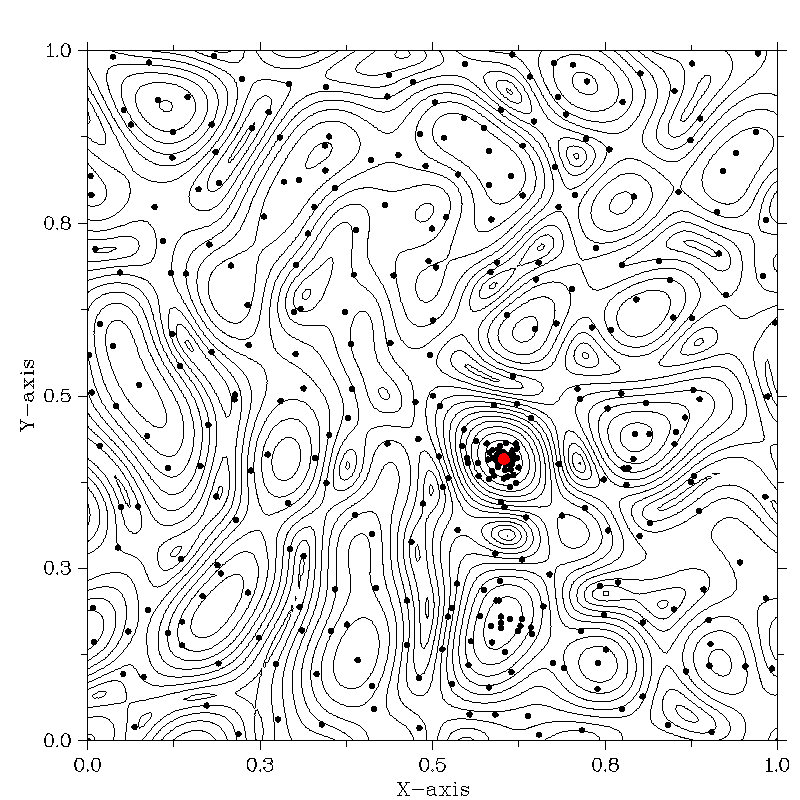
\includegraphics[width=.5\textwidth]{gs_loc.png}}}
  \subfloat[Пример линий уровня функции, порождённой GKLS]{
  {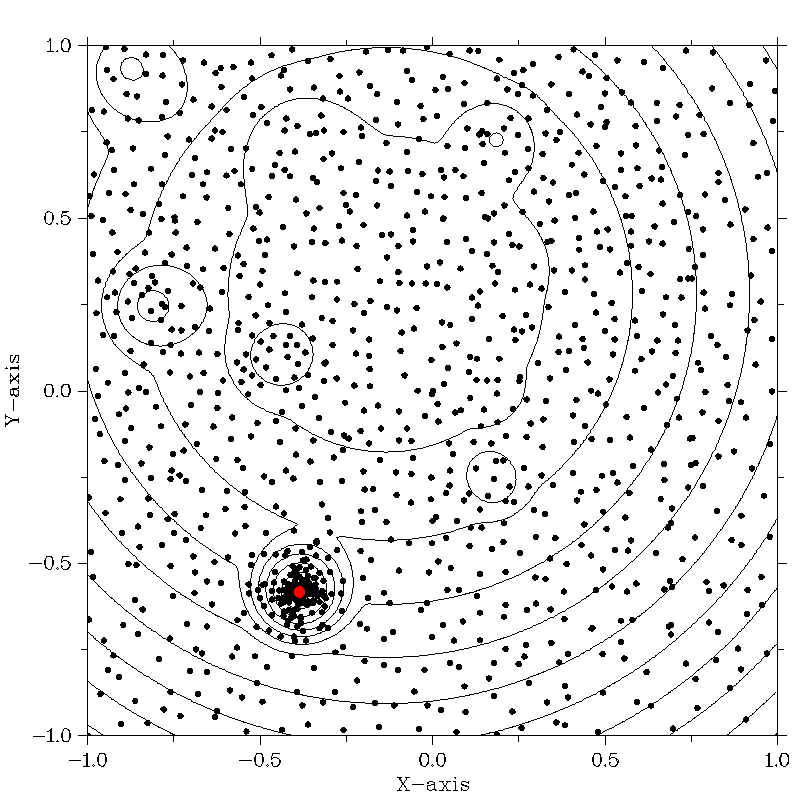
\includegraphics[width=.5\textwidth]{gkls_loc.png}}}
  \caption{Линии уровня и точки испытаний ИАГП в двух синтетических задачах без ограничений}
  \label{fig:isolines_unconstrained}
\end{figure}

Обозначим набор двумерных задач, полученный с помощью генератора \cite{grishaginClass}
как \(F_{GR}\). Генератор \(F_{GR}\) не позволяет контролировать размерность и сложность задач, а также количество локальных экстремумов.
Каждая тестовая задача определяется формулой:
\begin{displaymath}
  \varphi(y)=\sqrt{\left(\sum_{i=1}^7\sum_{j-1}^7 A_{ij}g_{ij}(y)+ B_{ij}h_{ij}(y)\right)^2+\left(\sum_{i=1}^7\sum_{j-1}^7 C_{ij}g_{ij}(y) - D_{ij}h_{ij}(y)\right)^2}
\end{displaymath}
где
\begin{displaymath}
  \begin{array}{cr}
    y\in[0;1]^2, \\
    g_{ij}=\sin(i\pi y_1)\sin(j\pi y_2), \\
    h_{ij}=\cos(i\pi y_1)\cos(j\pi y_2),
  \end{array}
\end{displaymath}
где коэффициенты \(A_{ij},B_{ij}, C_{ij}, D_{ij}\) генерируются случайно с равномерным в
интервале \([-1;1]\) распределением.
Получаемые функции являются существенно многоэксремальными. В данной работе будем использовать 100 функций, сненерированных с помощью \(F_{GR}\).

Геренатор GKLS \cite{Gaviano2003} позволяет получать тестовые задачи заданной размерности с заданным количеством локальных
экстремумов. Также этот генератор позволяет варьировать сложность задачи, изменяя размер области притяжения
глобального минимума. Это достигается за счёт модификации параболоида \(g(x)=\Vert x-T\Vert + t\) в
шаровых окрестностях некоторых случайно сгенерированных точек \(M_i, i=\overline{1,m}\). В точках
\(M_i\) располагаются локальные минимумы со значениями, превосходящими значение \(g(T)=t\).
В \cite{SergeyevKvasov2006} приводятся параметры генератора для получения 
наборов по 100 задач двух уровней сложности (Simple and Hard) размерностей 2, 3, 4 и 5.
Как и авторы генератора GKLS, будем использовать эти параметры и таким образом получим 800 тестовых задач.

Будем считать, что тестовая задача решена, если метод выполняет испытание
\(y^k\) в \(\delta\)-окрестности глобального минимума \(y^*\), т.е. $\left\|y^k-y^*\right\|_{inf}\leq \delta
= \alpha\left\|b-a\right\|_{inf}$, где \(a\) и \(b\) это правая и левая границы гиперкуба из (\ref{eq:task}),
а $\alpha$ это относительная точность. Если указанное соотношение не выполнено до исчерпания лимита на
испытания, то задача считается нерешённой. Лимит на количество испытаний и $\alpha$ заданы для каждого класса задач в отдельности
в соответствии с размерностью задач и их сложностью (see Table \ref{tab:limits}).

\begin{table}
\begin{center}
\caption{Лимит на количество испытаний и относительная точность в критерии остановки для различных классов задач}
  \begin{tabular}{|l|{c}|{c}|}
    \hline
  Problems class & Trials limit & $\alpha$\\
  \hline
  \(F_{GR}\) & 5000 & 0.01 \\
  \hline
  GKLS 2d Simple & 8000 & 0.01 \\
  \hline
  GKLS 2d Hard & 9000 & 0.01 \\
  \hline
  GKLS 3d Simple & 15000 & 0.01 \\
  \hline
  GKLS 3d Hard & 25000 & 0.01 \\
  \hline
  GKLS 4d Simple & 150000 & $\sqrt[4]{10^{-6}}$ \\
  \hline
  GKLS 4d Hard & 250000 & $\sqrt[4]{10^{-6}}$ \\
  \hline
  GKLS 5d Simple & 350000 & $\sqrt[5]{10^{-7}}$ \\
  \hline
  GKLS 5d Hard & 600000 & $\sqrt[5]{10^{-7}}$ \\
  \hline
  \end{tabular}
  \label{tab:limits}
\end{center}
\end{table}

Будем рассматривать среднее количество испытаний, затраченное на решение одной задачи, и количество
решенных задач как характеристики эффективности метода оптимизации на заданном классе задач.
Чем меньше среднее количество испытаний на задачу, тем быстрее метод сходится к решению, а значит и
меньше обращается к потенциально трудоёмкой процедуре вычисления ограничений и целевой функции задачи.
Количество решённых задач характеризует надёжность метода. Чтобы сделать рассматриваемые характеристики независимыми друг от друга,  
будем вычислять среднее количество испытаний, принимая во внимание только решённые задачи.

Среднее число испытаний на задачу в некоторых случаях не позволяет получить полной картины о
поведении численного метода оптимизации на рассматриваемом множестве задач. Например, если метод
тратит много ресурсов на решение небольшого подмножества задач из выборки, то это невозможно понять,
глядя только на среднее число испытаний. Как дополнительный критерий сравнения методов будем
использовать операционную характеристику \cite{grishaginClass}. Операционная характеристика
представляет из себя кривую на плоскости \((K, P)\), где \(K\) это среднее количество испытаний,
произведённое методом до выполнения критерия остановки, а \(P\) -- доля задач из выборки, решённых не более чем за \(K\)
испытаний. Если при заданном \(K\) операционная характеристика одного метода лежит выше, чем 
операционная характеристика другого, то это означает, что при фиксированных затратах на поиск,
первый метод с большей вероятностью найдёт решение. При заданном \(P\) если характеристика одного метода лежит левее, 
чем характеристика другого, то при одинаковой надёжности, первый метод в среднем потратит меньше испытаний на поиск, чем второй.
\section{Методы редукции размерности}
В этом разделе рассмотрим более подробно упомянутый ранее метод редукции размерности
с помощью кривых Пеано, заполняющих пространство, и сравним между собой разные модификации различных кривых.
Кроме прямой редукции размерности с помощью кривых типа Пеано, существует и способ, сводящий одну задачу оптимизации к
множеству вложенных задач оптимизации: многошаговая схема \cite{strongin1978}: 
\begin{equation}
  \label{eq:3}
  \min_{y \in D} \varphi(y) = \min_{y_1 \in [a_1, b_1]} \dots \min_{y_N \in [a_N, b_N]} \varphi(y_1, \dots, y_N).
\end{equation}

В рамках многошаговой схемы каждое вычисление целевой функции по переменной \(y_1\) во внешней задаче оптимизации влечёт за собой
проведение ещё \(N-1\) вложенной оптимизации. Недостатками данной схемы является её низкая экономичность в плане количества
обращений к целевой функции и отсутствие теоретической гаранитии сходимости IAGS при наличии функциональных ограничений
(в некоторых случаях целевые функции во вложенных задачах перестают удовлетворять условию Липшица). В качестве обобщения
многошаговой схемы было предложено вложенную оптимизацию вести не по одиночным переменным, а по блокам переменных \cite{globalizerSystem}.
К многомерным вложенным задачам в таком случае можно применить редукцию размерности с помощью кривых типа Пеано,
поэтому выявление наиболее эффективного типа кривой имеет смысл и для ускорения сходимости в случае блочной многошаговой схемы.

\subsection{Инъективная развёртка}

Для редукции размерности задач оптимизации в рамках информационно-статистического подхода
применяются кривые типа Пеано, заполняющие пространство (развёртки) \cite{Sergeyev2013, strongin1978,
Gergel2009, Strongin2000}. Такие кривые отображают
отрезок \([0,1]\) на \(N\)-мерный гиперкуб \(D\).

\par
После редукции размерности исходная многомерная задача (\ref{eq:task}) преобразуется в одномерную задачу
следующего вида:
\begin{equation}
\label{eq:oneDimTask}
\varphi(y(x^*))=\min\{\varphi(y(x)):x\in [0,1]\}.
\end{equation}
\par
Стоит отметить, что подстановка развёртки в Липшицеву функцию  % minimized
из (\ref{eq:task}) порождает одномерную функцию \(\varphi(y(x))\), которая удовлетворяет условию Гёльдера:
\begin{equation}
\label{eq:holder}
|\varphi(y(x_1))-\varphi(y(x_2))|\leq H{|x_1-x_2|}^{\frac{1}{N}}, x_1,x_2\in[0,1],
\end{equation}
где константа $H$ удовлетворяет неравенству \(H\leqslant2L\sqrt{N+3}\), \(L\) -- константа Липшица из (\ref{eq:lip}),
и \(N\) -- размерность задачи (\ref{eq:task}).
\par
Алгоритмы численного построения аппроксимаций кривой Пеано приведены в \cite{strSergGO}.

\par
Вычислительная схема алгоритма, применяющего кривые Пеано для редукции размерности, выглядит следующим образом:
\begin{itemize}
  \item Алгоритм оптимизации выполняет минимизацию редуцированной одномерной функции
  \(\varphi(y(x))\) из (\ref{eq:oneDimTask}),
  \item После нахождения точки следующего испытания \(x\), её многомерный образ \(y\)
  вычисляется с использованием развёртки \(y(x)\),
  \item Значение исходной многомерной функции \(\varphi(y)\) вычисляется в точке \(y\in D\),
  \item Вычисленное значение \(z=\varphi(y)\) используется как значение одномерной редуцированной функции \(\varphi(y(x))\) в точке \(x\).
\end{itemize}

%------------------------------------------------------------------------------
\subsection{Сдвиговые развёртки}
\label{sec:shifted}

Применение кривой типа Пеано для редукции размерности приводит к потере локальной информации об окрестности многомерных точек
в пространстве $\mathbb{R}^N$ (см. \cite{Strongin1992}).
Одним из способов частично решить эту проблему является использование множества развёрток \cite{Strongin1992}:
\begin{equation}%\label{eq:142}
Y_L(x)=\left\{y^0(x),\ y^1(x),...,\ y^L(x)\right\}
\end{equation}
вместо одной кривой Пеано $y(x)$ (см. \cite{Strongin1992,Strongin2000, Strongin1991}).

Такой набор отображений может быть получен путём сдвига исходной развёртки $y^0(x)$ на $2^{-l},0
\leq l \leq L$ по каждой из координат. Каждая из развёрток определена на своём гиперкубе $D_l=
\left\{y \in R^N: -2^{-1} \leq y_i+2^{-l} \leq 3 \cdot 2^{-1},\ 1\leq i\leq N\right\},\ 0 \leq l \leq
L$.

На Рис.~\ref{fig:shifted_ev} пунктирной линией обозначен образ интервала $[0,1]$, полученный с помощью $y^0(x),\
x\in [0,1],$. Поскольку гиперкуб $D$ из (\ref{eq:task}) принадлежит пересечению
семейства гиперкубов $D_l$, необходимо ввести дополнительное ограничение:
\begin{equation}\label{6_g0}
g_0(y)=\max\left\{\left|y_i\right| - 2^{-1}:\ 1\leq i\leq N\right\},
\end{equation}
тогда гиперкуб $D$ можно представить в виде
\[
D=\left\{y^l(x):\; x\in [0,1],\ g_0(y^l(x))\leq 0 \right\},\ 0\leq l \leq L,
\]
т.е. $g_0(y) \leq 0$ если $y\in D$, иначе $g_0(y)>0$. Следовательно, любая точка $y \in D$
имеет прообраз $x^l \in [0,1]$, определяемый соответствующей развёрткой $y^l(x),\ 0\leq l\leq L$.

Таким образом, каждая развёртка $y^l(x),\ 0\leq l \leq L,$ порождает свою собственную задачу вида
(\ref{eq:task}), имеющую расширенную (по сравнению с $D$) область поиска $D_l$
и дополнительное ограничение-неравенство с левой частью вида (\ref{6_g0})
\begin{equation}\label{6_problem_l}
\min{\left\{\varphi(y^l(x)):x\in [0,1], \; g_j(y^l(x))\leq 0, \; 0 \leq j \leq m\right\}}, \ 0 \leq l \leq L.
\end{equation}
При этом, $L$ копий метода AGS решают каждую из указанных задач, на каждой итерации обмениваясь многомерными точками
следующего испытания и добавляя их прообразы в свою поисковую информацию. Такая схема имеет смысл только при
наличии $L$ параллельных вычислительных ядер или процессоров.

\begin{figure}[ht]
    \centering
    \subfloat[Две сдвиговые развёртки, определённые на гиперкубах $D_0$ и $D_1$]{{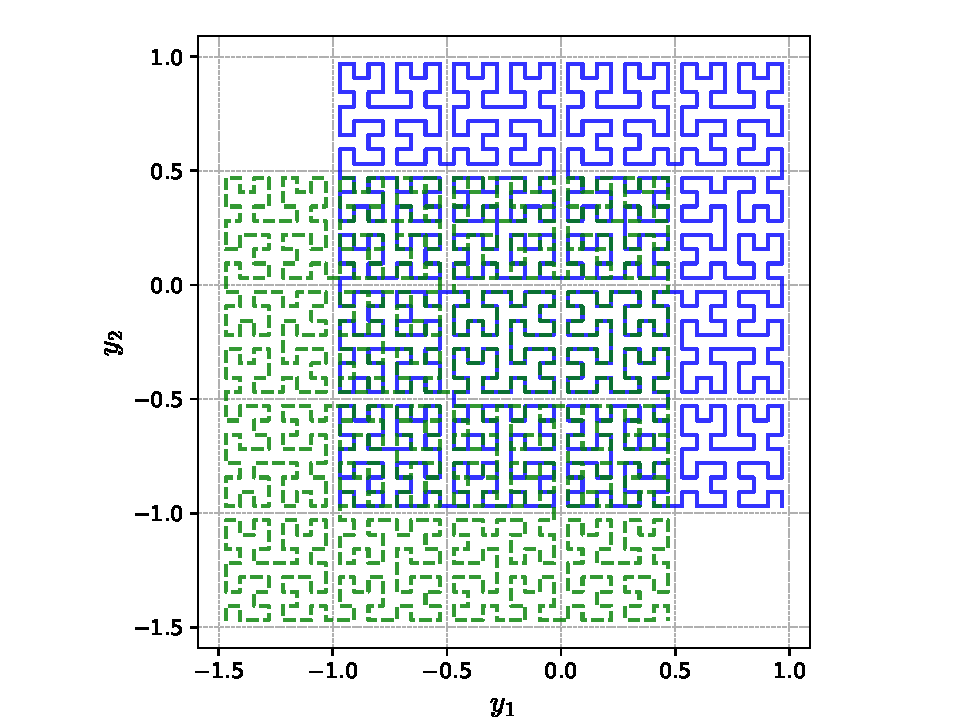
\includegraphics[width=.5\textwidth]{evolvents/shifted.pdf}}\label{fig:shifted_ev}}
    %\subfloat[Hypercubes $D_l$]{{\includegraphics[width=.4\textwidth]{pictures/shifted_cube.png}}\label{fig:shifted_cube}}
    \subfloat[Две вращаемые развёртки на одной плоскости]{{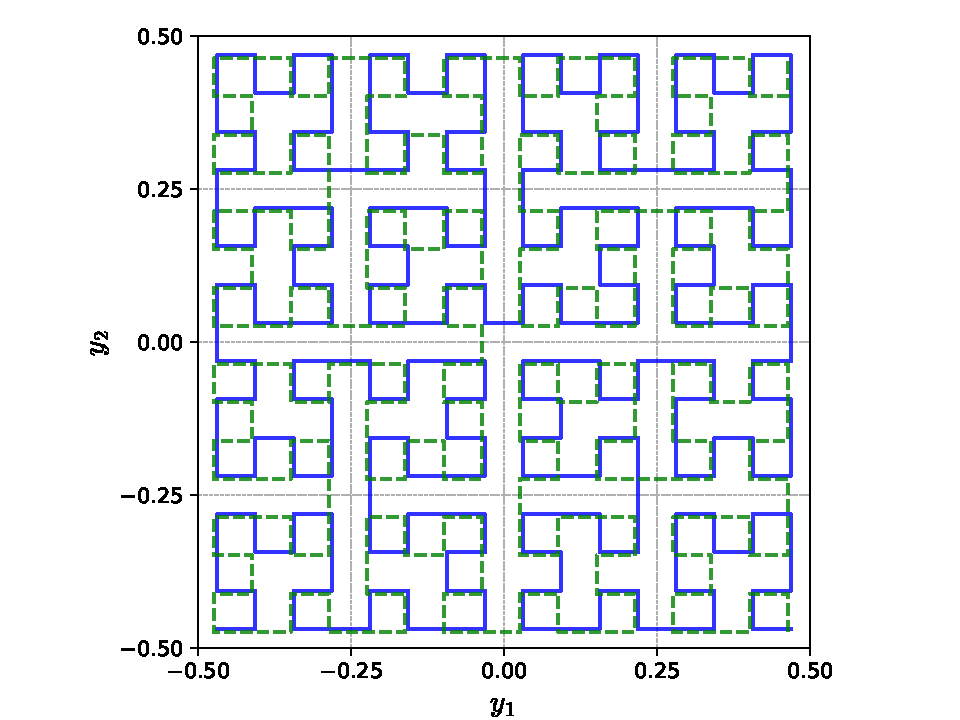
\includegraphics[width=.5\textwidth]{evolvents/rotated.pdf}}\label{6_fig_9}}
    \caption{Различные развёртки, построенные с низкой плотностью}
\end{figure}

%------------------------------------------------------------------------------
\subsection{Вращаемые развёртки}
Схема построения множества развёрток (здесь и далее будем называть, развёртки, порождённые ей сдвиговыми
или $S$-развёртками), описанная в Секции~\ref{sec:shifted}, позволяет сохранять часть информации
о близости точке в многомерном пространстве и, таким образом, обеспечивает более точную (по сравнению с одной развёрткой)
оценку константы Гёльдера в процессе оптимизации. Однако, однако, этот подход имеет недостаток в виде наличия дополнительного ограничения
что затрудняет построение эффективных реализаций алгоритма оптимизации на базе $S$-развёрток (см. конец Секции~\ref{sec:seq_comp}).

Чтобы обойти слложности, возникающие при работе с $S$-развёртками и одновременно сохранить часть иноррмации об окрестностях точек
$N$-мерном вещественном пространстве, была редложена ещё одна схема построения множества развёрток.
Эта схема предполагает вместо получения группы развёрток делать сдвиг не сдвиг кривой Пеано по диагонали гиперкуба, а
её вращение отностиельно центра координат \cite{Gergel2009}.
На Рис.~\ref{6_fig_9} представлены две развёртки, аппрокисимирующие привую Пеано при $N=2$.
Получая новые развёртки путём отражения относительно осей координат, можно породить множество развёрток
мощностью до $2^N$. При этом дополнительное ограничение $g_0(y)$ из (\ref{6_g0}), необходимое для получения
набора $S$-развёрток, отсутствует.
%Минусом вращаемых развёрток, по сравнению со сдвиговыми, является отсутствие теоретической гарантии
%получения близких прообразов для близких многомерных точек.
%Taking into account the initial mapping, one can conclude that current implementation of the

%------------------------------------------------------------------------------
\subsection{Неинъективная развёртка}

Как уже было сказано в секции \ref{sec:shifted}, потеря информации о близости точек в многомерном
пространстве может быть частично скомпенсирована использованием множественных отображений $Y_L(x)=\{y^1(x),...,y^L(x)\}$.
Однако, сама по себе кривая типа Пеано сохраняет в себе часть этой информации: она не является инъективым отображением,
поэтому имея один образ $y(x)\in \mathbb{R}^N$, можно получить несколько несколько отличных $x$ прообразов $t_j\in[0,1], t_j \not = x$,
которые затем могут быть добавлены в поисковую информацию индексного метода.

Кривая типа Пеано, используемая в (\ref{eq:oneDimTask}) для редукции размерности, определяется через предельный переход,
поэтому не может быть вычислена непосредтвенно. При численной оптимизации используется некоторое её приближение, являющееся
инъективной кусочно-линейной кривой. В \cite{strongin1978} было предложено неинъективное отображение равномерной сетки на
отрезка $[0,1]$ на равномерную сетку в гиперкубе $D$. Каждый многомерный узел может иметь до $2^N$ одномерных прообразов.
На рис. \ref{fig:noninjective} крестиками обозначена сетка в пространесве $\mathbb{R}^2$, для двух узлов которой
указаны соответствующие им одномерное прообразы из $[0,1]$ (отмечены квадратами и кругами). Каждый указанный узел имеет по 3 прообраза.

Недостатком неинъективной развёртки является потенциально большое количетво прообразов (до $2^N$).
% и невозможность использования параллельной схемы для множественных отображений из секции \ref{sec:parallel_evolvents}.


%------------------------------------------------------------------------------
\subsection{Гладкая развёртка}

Рассмотренные в предыдущих пунктах способы построения развертки строят кривую $y(x)$, которая не является
гладкой (см. рис. \ref{fig:shifted_ev}). Отсутствие гладкости может негативно сказаться на свойствах редуцированной
одномерной функции $\varphi(y(x))$, т.к. гладкая кривая более качественно передает информации о возрастании/убывании
исходной функции. На основе исходного алгоритма построения негладкой развертки было предложен обобщенный алгоритм
\cite{Goryachih2017}, позволяющий строить гладкую развёртку. Для иллюстрации на рис. \ref{fig:smooth} изображена гладкая
развертка в двумерном случае. Недостатком гладкой развёртки является в несколько раз большая сложность вычисления по
сравнению с кусочно-линейными кривыми (требуется вычислять нелинейные гладкие функции). Причём с ростом точности аппроксимации и
размерности количество интервалов гладкости увеличивается и сложность вычисления кривой нарастает.

\begin{figure}[ht]
    \centering
    \subfloat[Гладкая развёртка]{{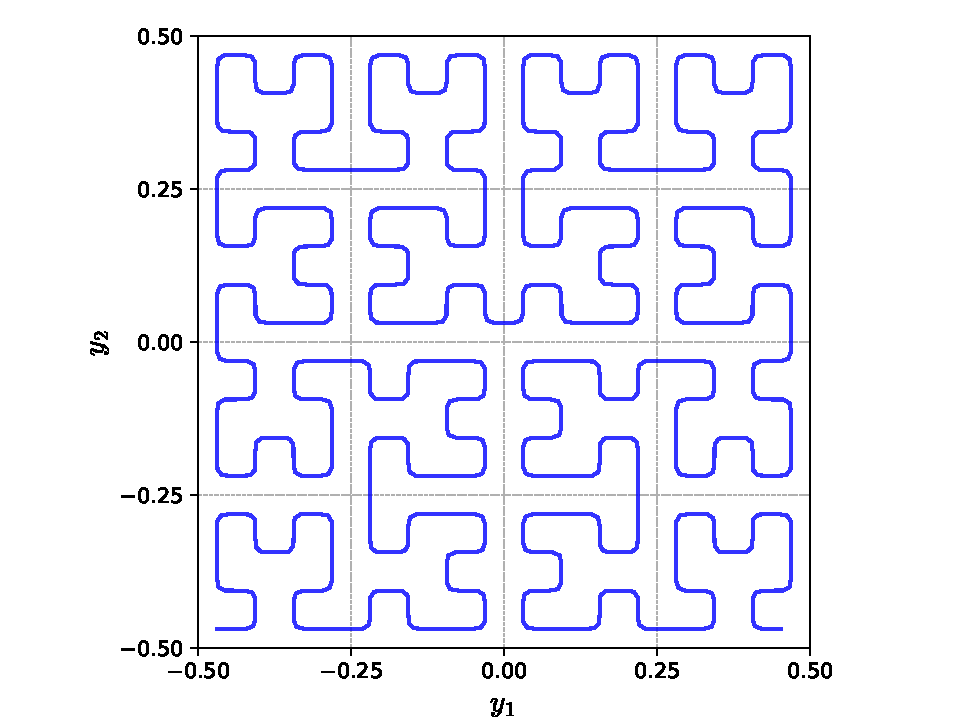
\includegraphics[width=.6\textwidth]{evolvents/smooth.pdf}}\label{fig:smooth}}
    \subfloat[Неинъективная развёртка]{{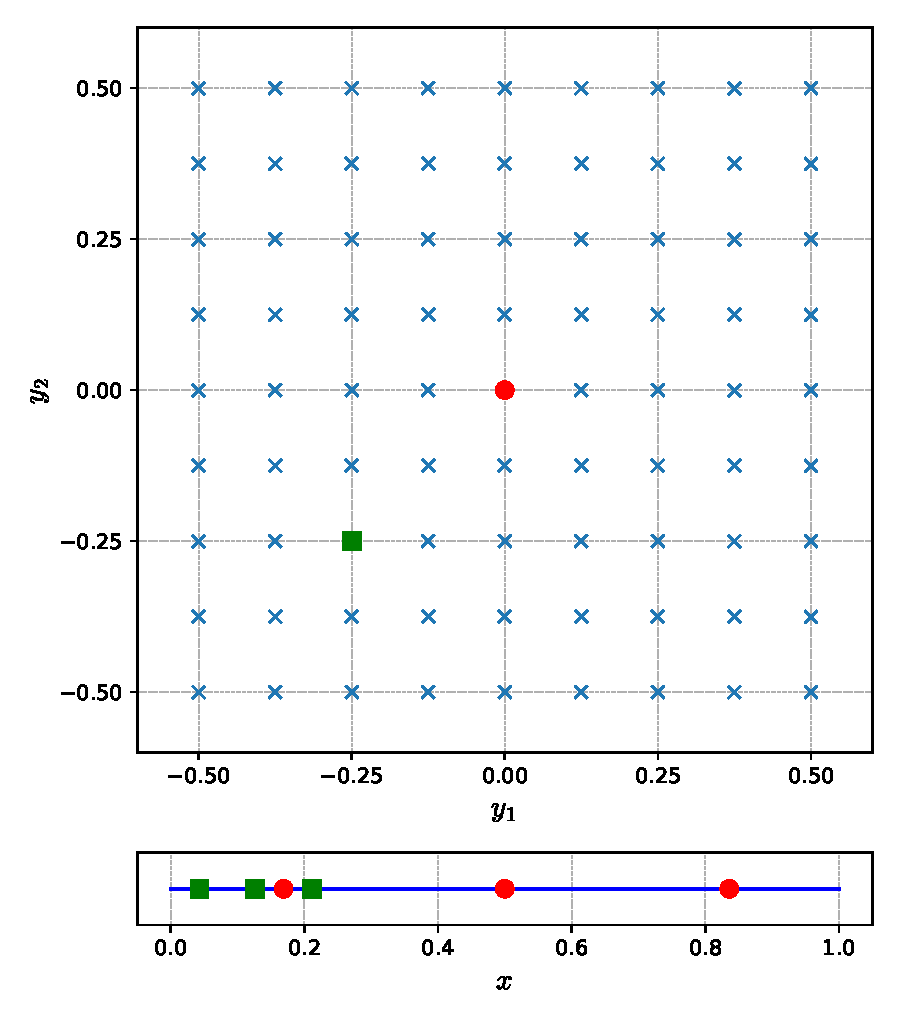
\includegraphics[width=.4\textwidth]{evolvents/noninjective.pdf}}\label{fig:noninjective}}
    \caption{Различные развёртки, построенные с низкой плотностью}
\end{figure}

\subsection{Сравнение развёрток}
\label{sec:seq_comp}
Сравнение скорости сходимости IAGS с различными типами развёткок проводилось в соответствии с методикой, описанной в
Секции \ref{sec:comp_tools}. С целью понять, обладает ли какой-либо из перечисленных ранее типов развёрток существенным преимуществом над другими,
были построены операционные характеристики индексного метода с различными типами развёрток на наборах задач GKLS 2d Simple и GKLS 3d Simple.

Во всех экспериментах параметр плотности построения развёрток $m=12$. Минимальное значение пераметра надёжности \(r\) было найдено
для каждого типа развёртки перебором по равномерной сетке с шагом \(0.1\).

На классе GKLS 2d Simple при минимальном \(r\) неинъективная и гладкая развёртка обеспечивают более быструю сходимость
(рис. \ref{fig:gkls2d_opt}). То же самое, наблюдается и при \(r=5.0\) (рис. \ref{fig:gkls2d_acc}). В последнем случае сдвиговая и
вращаемая развёртки начинают отставать от остальных, т.к. значение \(r=5.0\) является завышенным для них.
\begin{figure}[ht]
    \centering
    \subfloat[$r=5.0$]{{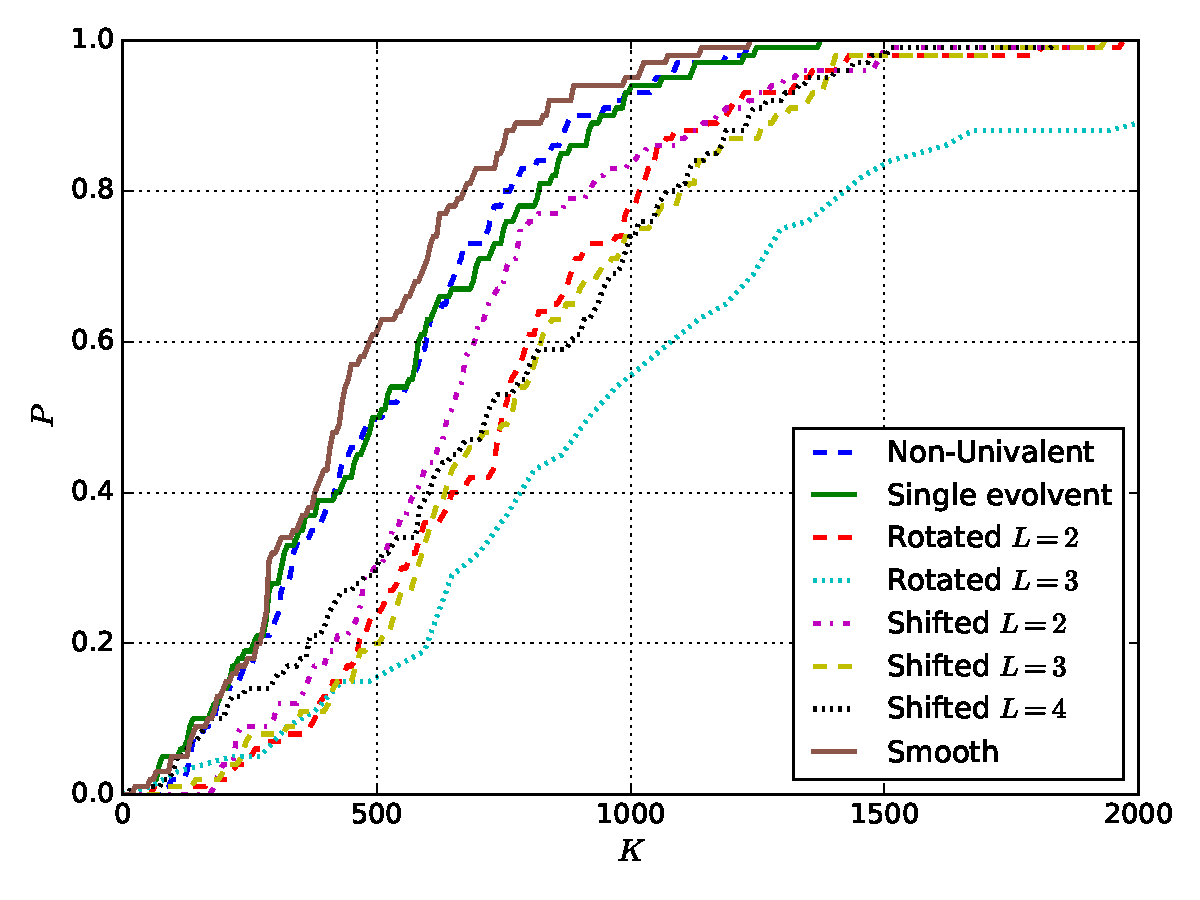
\includegraphics[width=.5\textwidth]{evolvents/gklsS2d_same_r_opt_pt_op.pdf}}\label{fig:gkls2d_acc}}
    \subfloat[Minimal $r$]{{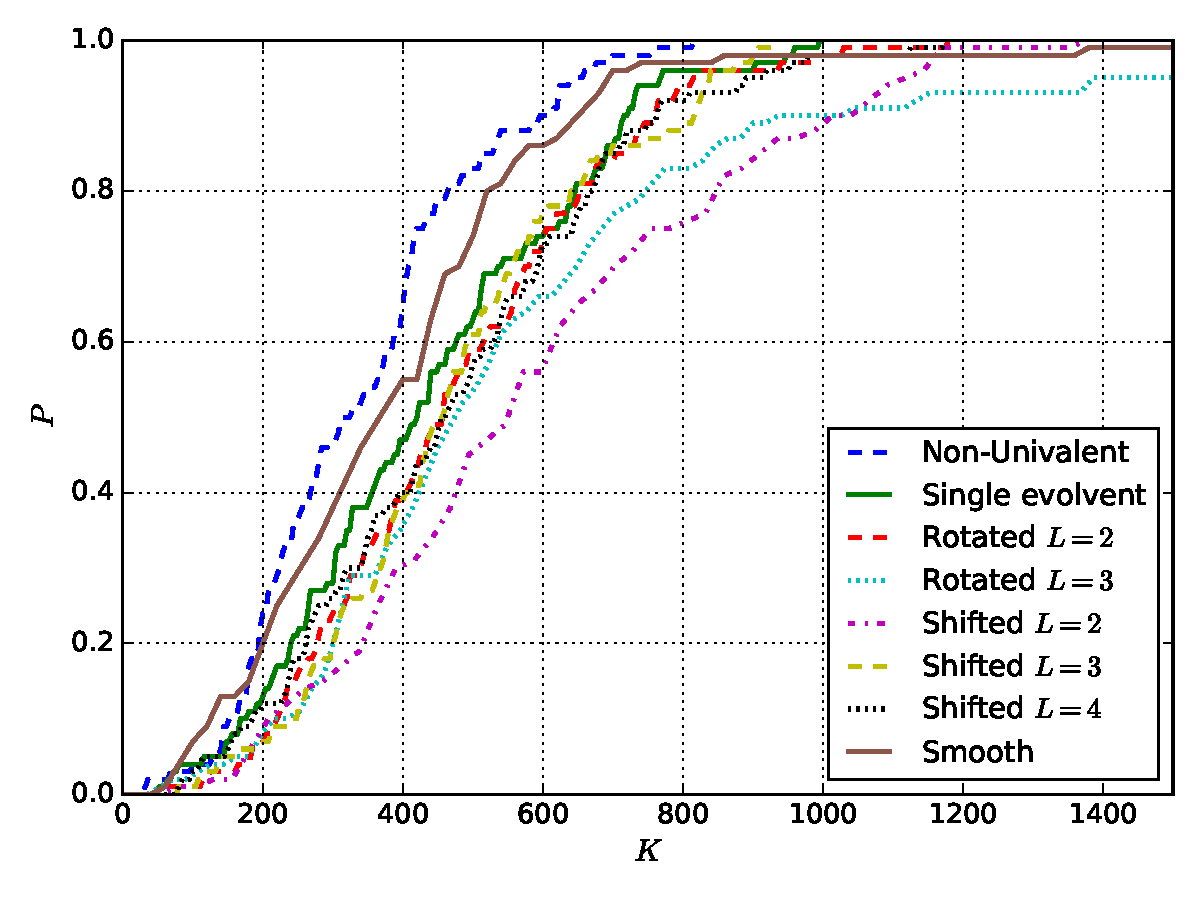
\includegraphics[width=.5\textwidth]{evolvents/gklsS2d_opt_pt_op.pdf}}\label{fig:gkls2d_opt}}
    \caption{Операционные характеристики на классе GKLS 2d Simple}
\end{figure}

На классе GKLS 2d Simple при минимальном \(r\) неинъективная и множественные развёртки имеют значительное
преимущество над единственной развёрткой (рис. \ref{fig:gkls3d_opt}). Значение \(r=4.5\) является завышенным для
вращаемой и сдвиговой развёрток (рис. \ref{fig:gkls3d_acc}).

\begin{figure}[ht]
    \centering
    \subfloat[$r=4.5$]{{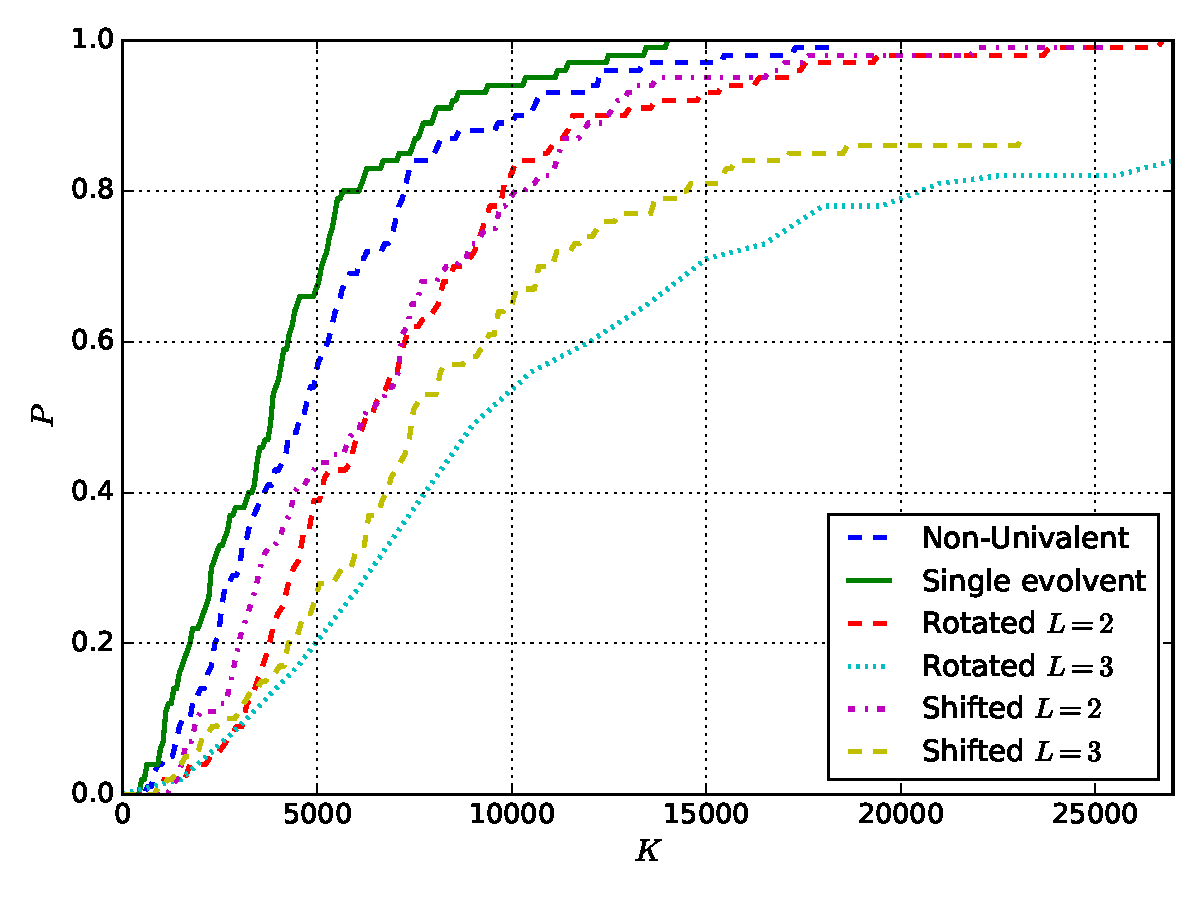
\includegraphics[width=.5\textwidth]{evolvents/gklsS3d_same_r_opt_pt_op.pdf}}\label{fig:gkls3d_acc}}
    \subfloat[Minimal $r$]{{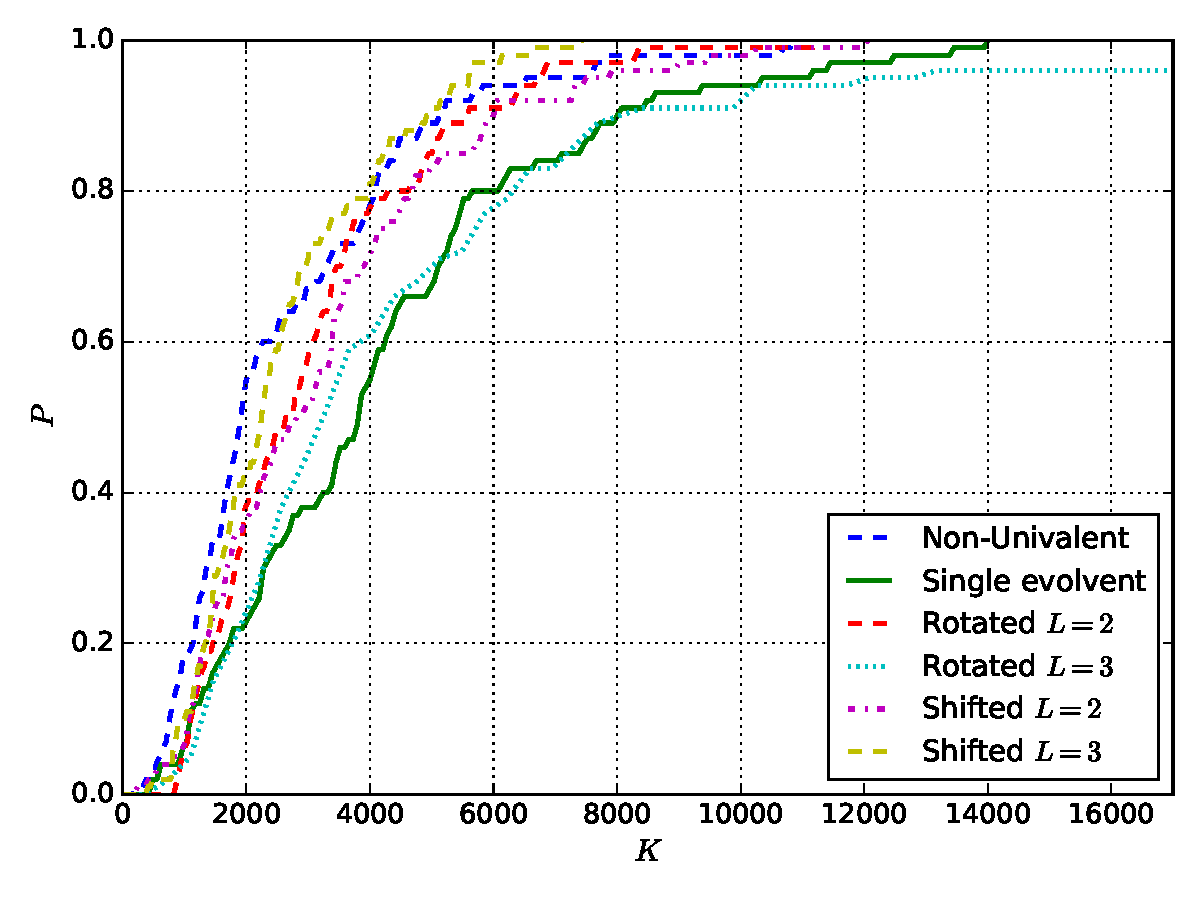
\includegraphics[width=.5\textwidth]{evolvents/gklsS3d_opt_pt_op.pdf}}\label{fig:gkls3d_opt}}
    \caption{Операционные характеристики на классе GKLS 3d Simple class}
\end{figure}

\paragraph{Накладные расходы при использовании сдвиговой развёртки.}
Во всех представленных выше экспериментах при построении операционной характеристики учитывалось количество
вычислений целевой функции из класса GKLS, однако в случае сдвиговой развёртки индексный метод решает задачу
с ограничением \(g_0\) из (\ref{6_g0}). В точках, где \(g_0\) нарушено, значение целевой функции не вычисляется.
Эти точки, тем не менее, хранятся в поисковой информации, создавая дополнительные расходы вычислительных ресурсов.
В таблице \ref{tab:shifted_g0} приведено среднее количество обращение к \(g_0\) и целевой функции. При \(L=3\)
ограниение \(g_0\) вычисляется почти в 20 раз чаще, чем целевая функция \(\varphi\), т. е. \(95\%\)
всей поисковой информации приходится на вспомогательные точки. Такие накладные расходы приемлемы при решении
задач малой размерности с трудоёмкими целевыми функциями, но при росте размерности и общего количества испытаний выгоднее
использовать другие типы развёрток.

\begin{table}
\begin{center}
\caption{Среднее количество вычислений \(g_0\) и \(\varphi\) при решении задач класса GKLS 3d Simple с помощью сдвиговой развёртки}
  \begin{tabular}{|l|{c}|{c}|{c}|}
    \hline
  $L$ & $calc(g_0)$ & $calc(\varphi)$ & $\frac{calc(g_0)}{calc(\varphi)}$ ratio \\
  \hline
  2 & 96247.9  & 6840.14 & 14.07\\
  \hline
  3 & 153131.0 & 7702.82 & 19.88\\
  \hline
  \end{tabular}
  \label{tab:shifted_g0}
\end{center}
\end{table}

\subsection{Итоги сравнения}

В результате проведённого сравнения различных способов редукции размерности, основанных на отображениях типа кривой Пеано,
можно сделать вывод о том, что для построения базовой весиии AGS с практической стороны
выгоднее использовать единственную кривую Пеано, кроме случаев низкой размерности или чрезвычайно трудоёмкого вычисления целевой
функции. Из множественных отображений оптимальным выбором будет использование вращаемых развёрток. Поскольку результаты, полученные для
алгоритма с одной развёрткой непосредственно распространяются на алгоритмы с вращаемыми развёртками, далее будем рассматривать
только случай единственной кривой Пеано.

\section{Review of Considered Optimization Methods}
\subsubsection{Hyperparameters control in AGS}

The parameter $r$ from (\ref{eq:step2}) affects the global convergence of AGS directly (see
\cite{strSergGO}, Chapter 8):
at high enough value of $r$, the method converges to all global minima of the objective function with
guarantee.
At the same time, according to (\ref{eq:step3_2}) and (\ref{step5}), at the infinitely high value of $r$, AGS turns into
the brute force search method on a uniform grid.

In the ideal case, in order to provide the highest convergence speed, the estimate of the Lipschitz
constant from (\ref{eq:step2})
should not be too overestimated, but in practice the actual value of $L$ from (\ref{eq:lip}) in
unknown, and one has either to take an obviously overestimated value of $r$ or to execute several
runs of AGS with different parameters. In order to resolve the problem of choosing $r$ to some extent,
let us use the following scheme:
\begin{itemize}
  \item execute $q$ iterations of AGS with $r=r_{max}$;
  \item execute $q$ iterations of AGS with $r=r_{min}$;
  \item repeat the above steps either until convergence or until the allowed number of iterations are
exhausted.
\end{itemize}

In the above algorithm, $r_{min} < r_{max}$, $q > 1$. Instead one parameter $r$, now
3 ones should be selected. However, according to the results of the numerical experiments, it is easier
than to find the optimal value of $r$.
Intuitively, the practical efficiency of the proposed scheme can be explained by the fact that now the
operation of the method takes place in two modes: the global search with $r=r_{max}$ and the local
one with $r=r_{min}$. If during the global search phase, the method approached the global minimum
whereas during the next phase, the estimate of the global minimum  would be refined rapidly.
If two phases are not enough, the process is continued. This way, a better trade-off
between the exploration and the exploitation is achieved.
Further, we will denote the method utilizing the scheme described above as AGS-AR.

\subsection{Other Optimization Methods}
\begin{itemize}
  \item \textbf{Multi Level Single Linkage} \cite{Kan1987StochasticGO}. MLSL is an improved
multistart algorithm.
  It samples low-discrepancy starting points and does local optimizations from them. In contrast to
the dummy multistart schemes
  MLSL uses some clustering heuristics to avoid multiple local descents to already explored local
minima.

  \item \textbf{DIRECT} \cite{Jones2009}. The algorithm is deterministic and recursively divides
the search space and forms a tree of hyper-rectangles (boxes). DIRECT uses the objective function
values and the Lipschitz condition (\ref{eq:lip}) to estimate promising boxes.

  \item \textbf{Locally-biased DIRECT (DIRECT$l$)} \cite{Gablonsky2001}. It's a variation of
DIRECT which pays less attention to non-promising boxes and therefore
  has less exploration power: it can converge faster on problems with few local minima, but lost the
global one in complicated cases.

  \item \textbf{Dual Simulated Annealing} \cite{XIANG1997216}. This stochastic method is a
combination of the Classical Simulated Annealing and the Fast Simulated Annealing coupled to a
strategy for applying a local search on accepted locations. It converges much faster than both parent
algorithms, CSA and FSA.

  \item \textbf{Differential Evolution} \cite{Storn1997}. DE is an adaptation of the original genetic
algorithm to
  the continuous search domain.

  \item \textbf{Controlled Random Search} \cite{Price1983}. The CRS starts with a set of random
points and then defines
  the next trial point in relation to a simplex chosen randomly from a stored configuration of points.
CRS in not an
  evolutional algorithm, although stores something like population and performs transformation
resembling a mutation.

  \item \textbf{StoGO} \cite{Madsen1998}. StoGO is dividing the search space into smaller hyper-
rectangles via a branch-and-bound approach,
  and searching them by a local-search algorithm, optionally including some randomness.

\end{itemize}

All the mentioned algorithms are available in source codes as parts of wide-spread optimization packages.
DIRECT, DIRECT$l$, CRS, MLSL and StoGO are part of the NLOpt library \cite{nlopt}.
Differential Evolution and DSA can be found in
the latest version of the SciPy \cite{scipy} package for Python.

\section{Tools for Comparison of Global Optimization Algorithms}

The use of the sets of test problems with known solutions generated by some random mechanisms is
one of commonly accepted approaches to comparing the optimization algorithms
\cite{Beiranvand2017}. In the present work, we will use two generators of test problems generating
the problems of different nature \cite{grishaginClass, Gaviano2003} \footnote{Software implementations of
these generators are available in source codes at the page \url{https://github.com/sovrasov/global-optimization-test-problems}}.

Let us denote the problem set obtained with the use of the first generator from \cite{grishaginClass}
as \(F_{GR}\). The mechanism of generation of the problems \(F_{GR}\) doesn't provide the
control of the problem complexity and of the number of local optima. However, the generated
functions are known to be the multiextremal ones essentially. Besides, the problems generated by
\(F_{GR}\) are the two-dimensional ones. In the present work, we will use 100 functions from the
class \(F_{GR}\) generated randomly.

The GKLS generator \cite{Gaviano2003} allows obtaining the problems of given dimensionality
with given number of extrema. Moreover, GKLS allows adjusting the complexity of the problems by
decreasing or increasing the size of the global minimum attractor. In
\cite{SergeyevKvasov2006} the parameters of the generator allowing generating the sets of 100
problems each of two levels of complexity (Simple and Hard) of the dimensionality equal to 2, 3, 4,
and 5 are given. Following the authors of the GKLS generator, we will use the parameters proposed
by them and, this way, add 800 more problems of various dimensionalities and complexity into the
test problem set.

Let us suppose a test problem to be solved if the optimization method executes the scheduled trial
\(y^k\) in a \(\delta\)-vicinity of the global minimum \(y^*\), i.e. $\left\|y^k-y^*\right\|\leq \delta
= \alpha\left\|b-a\right\|$, where \(a\) and \(b\) are the left and the right boundaries of the hypercube
from (\ref{eq:task}), $\alpha$ is relative precision. If this relation is not fulfilled before the expiration of the limit of the number of
trials, the problem was considered to be unsolved. The limit of the number of trials and $\alpha$ were set
for each problem class according to the dimensionality and complexity (see Table \ref{tab:limits}).

\begin{table}
\begin{center}
\caption{Trials limits and relative precision for the test problem classes}
  \begin{tabular}{|l|{c}|{c}|}
    \hline
  Problems class & Trials limit & $\alpha$\\
  \hline
  \(F_{GR}\) & 5000 & 0.01 \\
  \hline
  GKLS 2d Simple & 8000 & 0.01 \\
  \hline
  GKLS 2d Hard & 9000 & 0.01 \\
  \hline
  GKLS 3d Simple & 15000 & 0.01 \\
  \hline
  GKLS 3d Hard & 25000 & 0.01 \\
  \hline
  GKLS 4d Simple & 150000 & $\sqrt[4]{10^{-6}}$ \\
  \hline
  GKLS 4d Hard & 250000 & $\sqrt[4]{10^{-6}}$ \\
  \hline
  GKLS 5d Simple & 350000 & $\sqrt[5]{10^{-7}}$ \\
  \hline
  GKLS 5d Hard & 600000 & $\sqrt[5]{10^{-7}}$ \\
  \hline
  \end{tabular}
  \label{tab:limits}
\end{center}
\end{table}

Let us consider the averaged number of trials executed to solve a single problem and the number of
solved problems as the characteristics of the optimization method on each class. The less the number
of trials, the faster the method converges to a solution, hence the less times it turns to a potentially
computation-costly procedure of computing the objective function. The number of solved problems
evidences the reliability of the method at given parameters on the class of test problems being
solved. In order to make independent the quantities featuring the reliability and the speed of convergence,
averaged number of trials always was calculated taking into account solved problems only.

The average number of trials doesn't represent the real behavior of an optimization method
on a problems set in some cases. For an instance, if a method performs well on the most problems
and spends too much trials to solve the least several problems, we wouldn't catch such
case looking at the average number of trials only.
As an advanced measure of performance we will use the operating characteristic \cite{grishaginClass}.
It's defined by a set of points on the \((K, P)\) plane where \(K\) is the average number of search trials
conducted before satisfying the termination condition when minimizing a function
from a given class, and \(P\) is the proportion of problems solved successfully.
If at a given \(K\), the operating characteristic of a method goes higher than one
from another method, it means that at fixed search costs, the former method has a
greater probability of finding the solution. If some value of \(P\) is fixed, and the
characteristic of a method goes to the left from that of another method, the former
method requires fewer resources to achieve the same reliability.

\section{Results of Numerical Experiments}
\label{sec:experiments}
The results of various algorithms on different problem classes depend on the adjustments of
algorithms directly. In most cases, the authors of software implementations are oriented onto the
problems of medium difficulty. In order to obtain a satisfactory result when solving the essentially
multiextremal problems, a correction of some parameters is required. When conducting the
comparison, the following parameters for the methods were employed:
\begin{itemize}
  \item in the AGS-AR method, the parameter of alternation the
  global and local stages $q$ was set to be equal to $50\cdot\log_2(N-1)\cdot N^2$, also $r_{min}=3,\:r_{max}=2\cdot r_{min}$;
  \item in the DIRECT and DIRECT\(l\) methods, the parameter \(\epsilon=10^{-4}\);
  \item in the SDA method, the parameter \(visit=2.72\).
\end{itemize}

The rest parameters were varied subject to the problem class (see Table \ref{tab:params}).
For the AGS the value ot the $r$ parameter, such that the method solves all problems and performs the minimum amount of trials,
was estimated by brute force on the uniform grid with step $0.1$.

\begin{table}
\begin{center}
\caption{Class-specific parameters of the optimization algorithms}
  \begin{tabular}{|l|{c}|{c}|{c}|}
    \hline
    & AGS & CRS & DE\\
  \hline
  \(F_{GR}\) & \(r=3\) & popsize=150 & mutation=(1.1,1.9), popsize=60 \\
  \hline
  GKLS 2d Simple & \(r=4.6\) & popsize=200 & mutation=(1.1,1.9), popsize=60 \\
  \hline
  GKLS 2d Hard & \(r=6.5\) & popsize=400 & mutation=(1.1,1.9), popsize=60 \\
  \hline
  GKLS 3d Simple & \(r=3.7\) & popsize=1000 & mutation=(1.1,1.9), popsize=70 \\
  \hline
  GKLS 3d Hard & \(r=4.4\) & popsize=2000 & mutation=(1.1,1.9), popsize=80 \\
  \hline
  GKLS 4d Simple & \(r=4.7\) & popsize=8000 & mutation=(1.1,1.9), popsize=90 \\
  \hline
  GKLS 4d Hard & \(r=4.9\) & popsize=16000 & mutation=(1.1,1.9), popsize=100 \\
  \hline
  GKLS 5d Simple & \(r=4\) & popsize=25000 & mutation=(1.1,1.9), popsize=120 \\
  \hline
  GKLS 5d Hard & \(r=4\) & popsize=30000 & mutation=(1.1,1.9), popsize=140 \\
  \hline
\end{tabular}
  \label{tab:params}
\end{center}
\end{table}

\begin{table}
\begin{center}
\caption{Averaged number of trials executed by optimization methods for solving the test
optimization problems}
\resizebox{\textwidth}{!}{%
  \begin{tabular}{|l|{c}|{c}|{c}|{c}|{c}|{c}|{c}|{c}|{c}|{c}|}
    \hline
    & AGS & AGS-AR & CRS & DIRECT & DIRECT\(l\) & MLSL & SDA & DE & StoGO \\
  \hline
  \(F_{GR}\)     & 193.1 & 248.3 & 400.3 & \textbf{182.2} & 214.9 & 947.2 & 691.2 & 1257.3 & 1336.8 \\
  \hline
  GKLS 2d Simple & 254.9 & 221.6 & 510.6 & \textbf{189.0} & 255.2 & 556.8 & 356.3 & 952.2 & 1251.5 \\
  \hline
  GKLS 2d Hard   & \textbf{728.7} & 785.0 & 844.7 & 985.4 & 1126.7 & 1042.5 & 1637.9 & 1041.1 & 2532.2 \\
  \hline
  GKLS 3d Simple &  1372.1 & 1169.5 & 4145.8 & \textbf{973.6} & 1477.8 & 4609.2 & 2706.5 & 5956.9 & 3856.1 \\
  \hline
  GKLS 3d Hard   &  3636.1 & \textbf{1952.1} & 6787.0 & 2298.7 & 3553.3 & 5640.1 & 4708.4 & 6914.3 & 7843.2 \\
  \hline
  GKLS 4d Simple &  5729.8 & \textbf{4919.1} & 19883.6 & 7328.8 & 15010.0 & 41484.8 & 22066.0 & 6271.2 & 29359.2 \\
  \hline
  GKLS 4d Hard   &  13113.4 & \textbf{12860.1} & 27137.4 & 22884.4 & 55596.1 & 80220.1 & 68048.0 & 12487.6 & 58925.5  \\
  \hline
  GKLS 5d Simple &  \textbf{5821.5} & 6241.3 & 62921.7 & 5966.1 & 10795.5 & 52609.2 & 34208.8 & 20859.4 & 69206.8 \\
  \hline
  GKLS 5d Hard   &  \textbf{17008.6} & 21555.1 & 87563.9 & 61657.3 & 148637.8 & 138011.8 & 115634.6 & 26850.0 & 141886.5 \\
  \hline
\end{tabular}}
  \label{tab:trials}
\end{center}
\end{table}

The results of running the optimization methods on the considered problem classes are presented in
Tables \ref{tab:trials}, \ref{tab:solved}. The DIRECT, AGS and AGS-AR methods have demonstrated the
best convergence speed on all classes, at that AGS-AR inferior to DIRECT on the 2d problems from the
Simple classes and has an advantage on the problems of the Hard classes. As one can see from Table
\ref{tab:solved}, the deterministic methods (AGS, AGS-AR, DIRECT, and DIRECT\(l\)) were the
most reliable. Among the stochastic methods, MLSL and SDA have demonstrated the highest
reliability.

\begin{table}
\begin{center}
\caption{Number of test optimization problems solved by the methods}
  \begin{tabular}{|l|{c}|{c}|{c}|{c}|{c}|{c}|{c}|{c}|{c}|{c}|}
    \hline
    & AGS & AGS-AR & CRS & DIRECT & DIRECT\(l\) & MLSL & SDA & DE & StoGO \\
  \hline
  \(F_{GR}\)     &  100 & 100 & 76 & 100 & 100 & 97 & 96 & 96 & 67\\
  \hline
  GKLS 2d Simple &  100 & 100 & 85 & 100 & 100 & 100 & 100 & 98 & 90\\
  \hline
  GKLS 2d Hard   &  100 & 97 & 74 & 100 & 100 & 100 & 93 & 85 & 77 \\
  \hline
  GKLS 3d Simple &  100 & 100 & 75 & 100 & 100 & 100 & 89 & 86 & 44 \\
  \hline
  GKLS 3d Hard   &  100 & 100 & 72 & 100 & 99 & 100 & 88 & 77 & 43 \\
  \hline
  GKLS 4d Simple &  100 & 100 & 74 & 100 & 100 & 94 & 82 & 68 & 72 \\
  \hline
  GKLS 4d Hard   &  100 & 100 & 60 & 99 & 99 & 94 & 73 & 55 & 69  \\
  \hline
  GKLS 5d Simple &  100 & 100 & 86 & 100 & 100 & 98 & 100 & 88 & 82  \\
  \hline
  GKLS 5d Hard   &  100 & 100 & 77 & 100 & 93 & 79 & 86 & 77 & 78 \\
  \hline
  \end{tabular}
  \label{tab:solved}
\end{center}
\end{table}

\begin{figure}[ht]
  \centering
  \subfloat[4d Simple]{{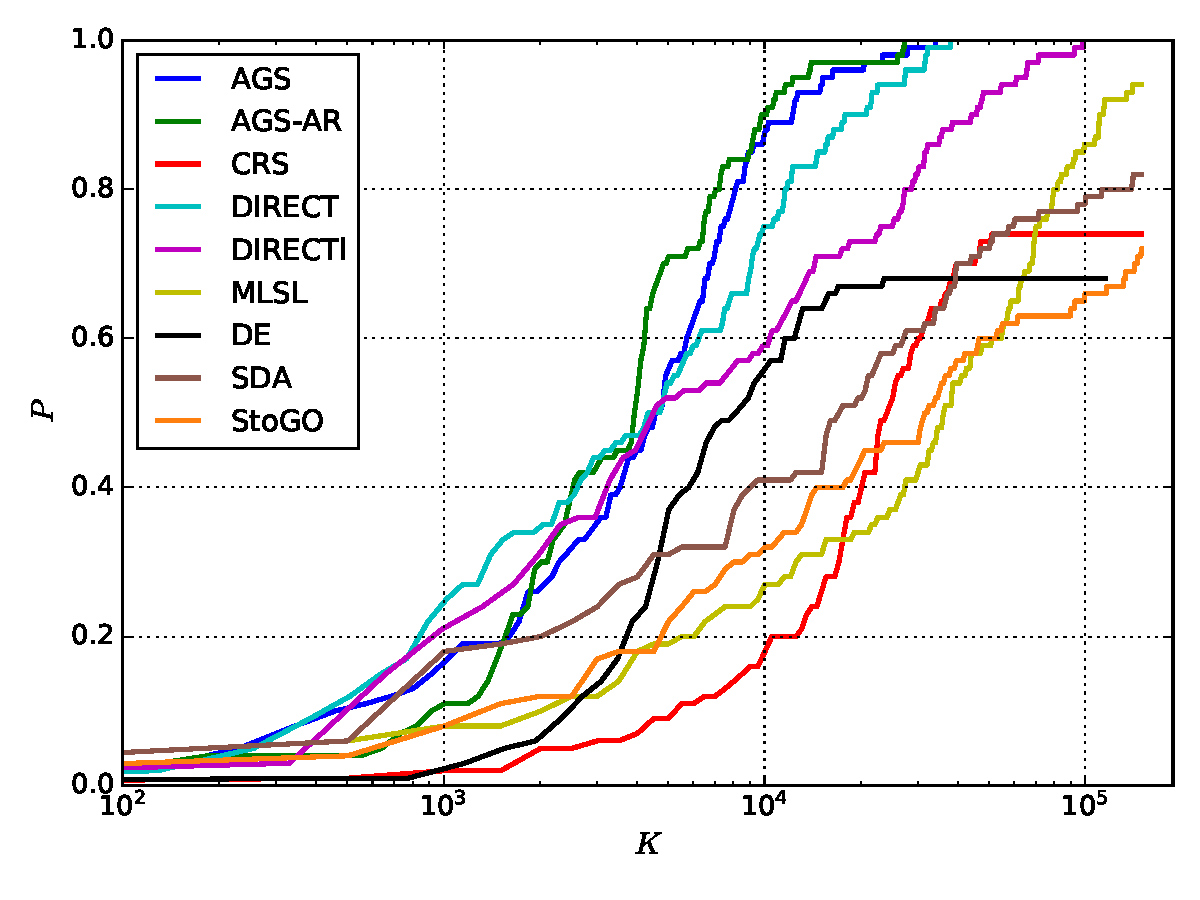
\includegraphics[width=.5\textwidth]{images/gklss4d.pdf}}\label{fig:s4d}}
  \subfloat[4d Hard]{{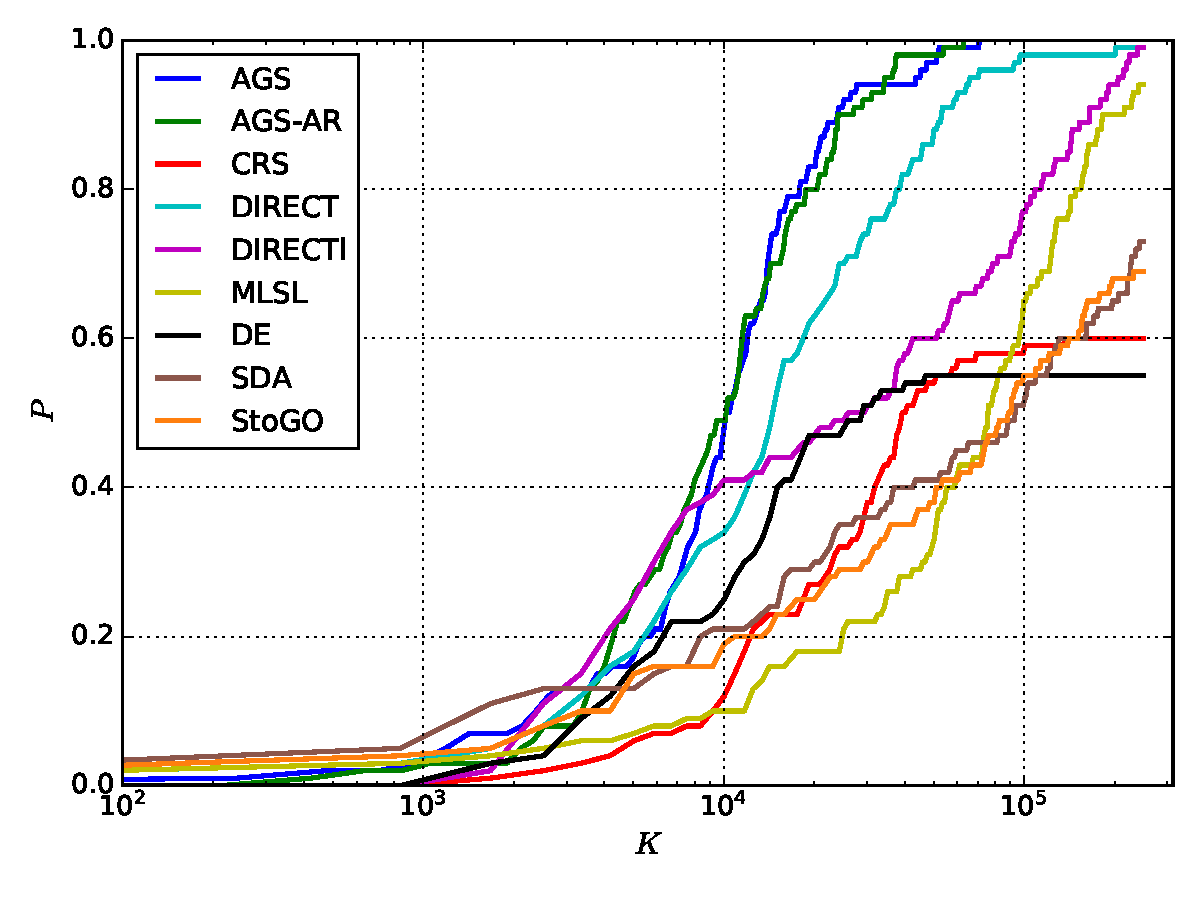
\includegraphics[width=.5\textwidth]{images/gklsh4d.pdf}}\label{fig:h4d}}

  \subfloat[5d Simple]{{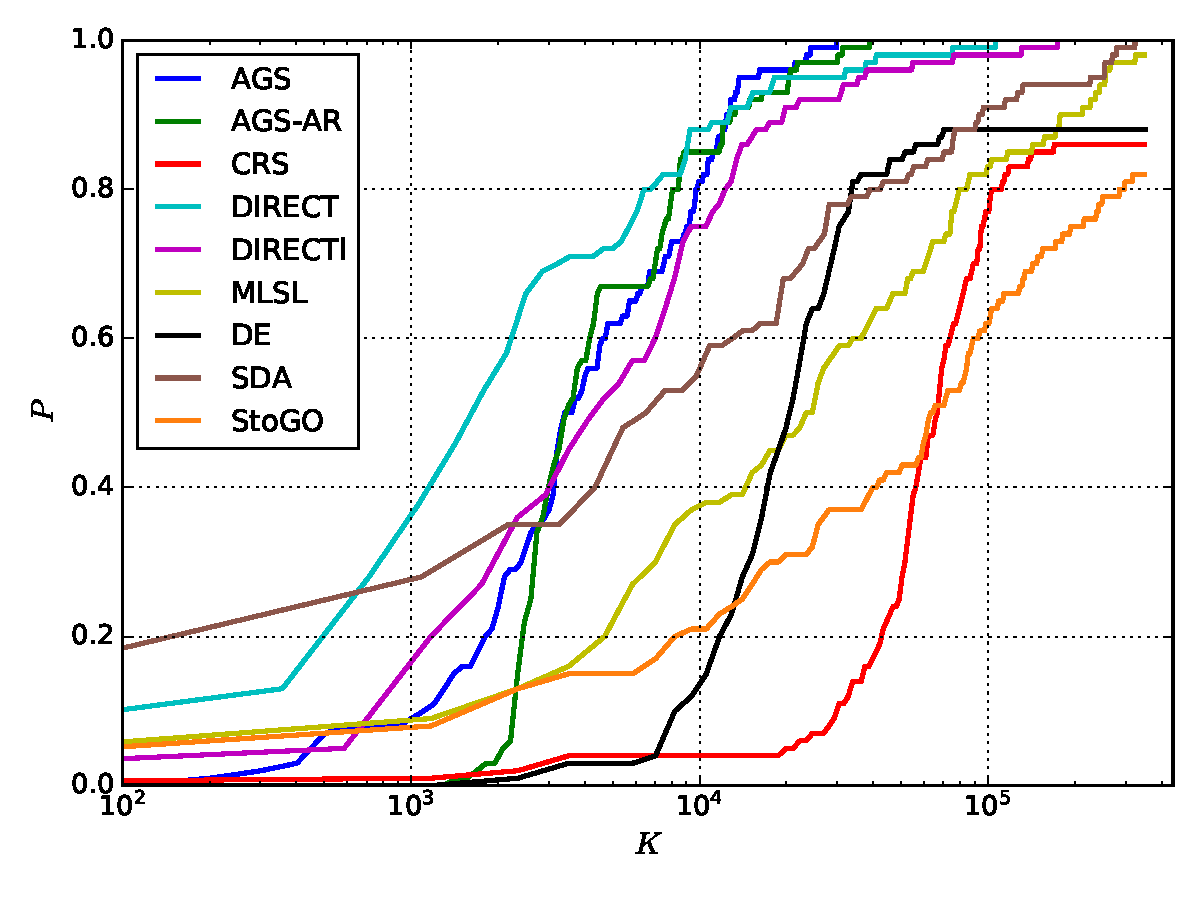
\includegraphics[width=.5\textwidth]{images/gklss5d.pdf}}\label{fig:s5d}}
  \subfloat[5d Hard]{{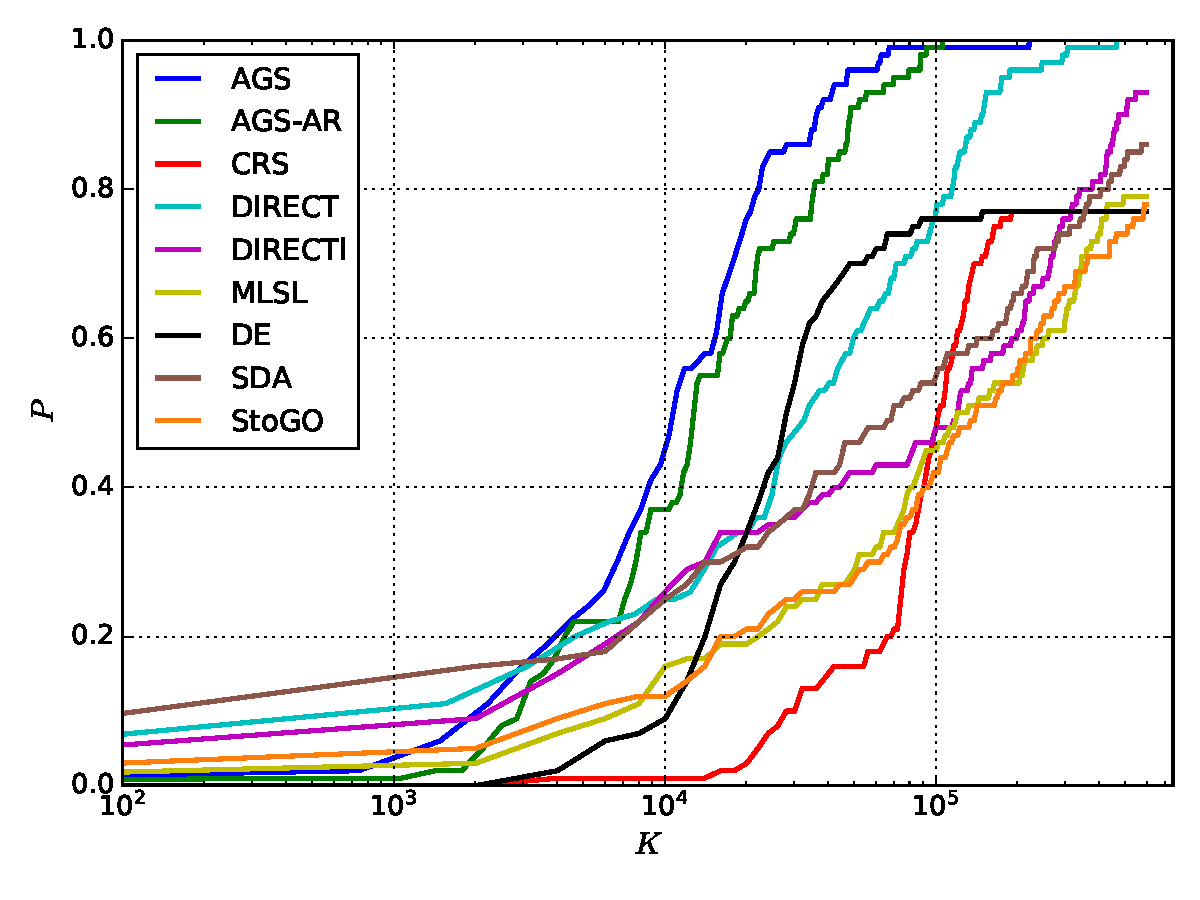
\includegraphics[width=.5\textwidth]{images/gklsh5d.pdf}}\label{fig:h5d}}
  \caption{Operating characteristics of the algorithms when solving problems from the GKLS 4d and 5d classes. Best viewed in color.}
\end{figure}

Operating characteristic of the methods (Figures \ref{fig:s4d}, \ref{fig:h4d}, \ref{fig:s5d}, \ref{fig:h5d})
demonstrates that AGS and AGS-AR faster than the other methods achieve 100\% success rate. Also on GKLS 5d Simple the DIRECT
generally has the best performance, but there are several hard problems that affect it's average number of
trials metric.

\paragraph{Robustness of AGS and AGS-AR to the Hyperparameters Choice.}

In order to investigate the influence of hyperparameters to the convergence speed of the AGS and AGS-AR,
experiments with the following settings were conducted on the problems from GKLS 5d Simple class:
\begin{itemize}
  \item AGS with $r=4$ (like in the Table \ref{tab:params});
  \item AGS with $r=6$;
  \item AGS-AR with parameters from the beginning of the Section \ref{sec:experiments}
  ($q=50\cdot\log_2(4)\cdot 25 = 2500$, $r_{min}=3,\:r_{max}=2\cdot r_{min}$);
  \item AGS-AR with $r_{max}=8$ and other parameters from the previous experiment;
  \item AGS-AR with $q=1000$ and other parameters from the beginning of the Section \ref{sec:experiments};
\end{itemize}

\begin{figure}[ht]
  \centering
  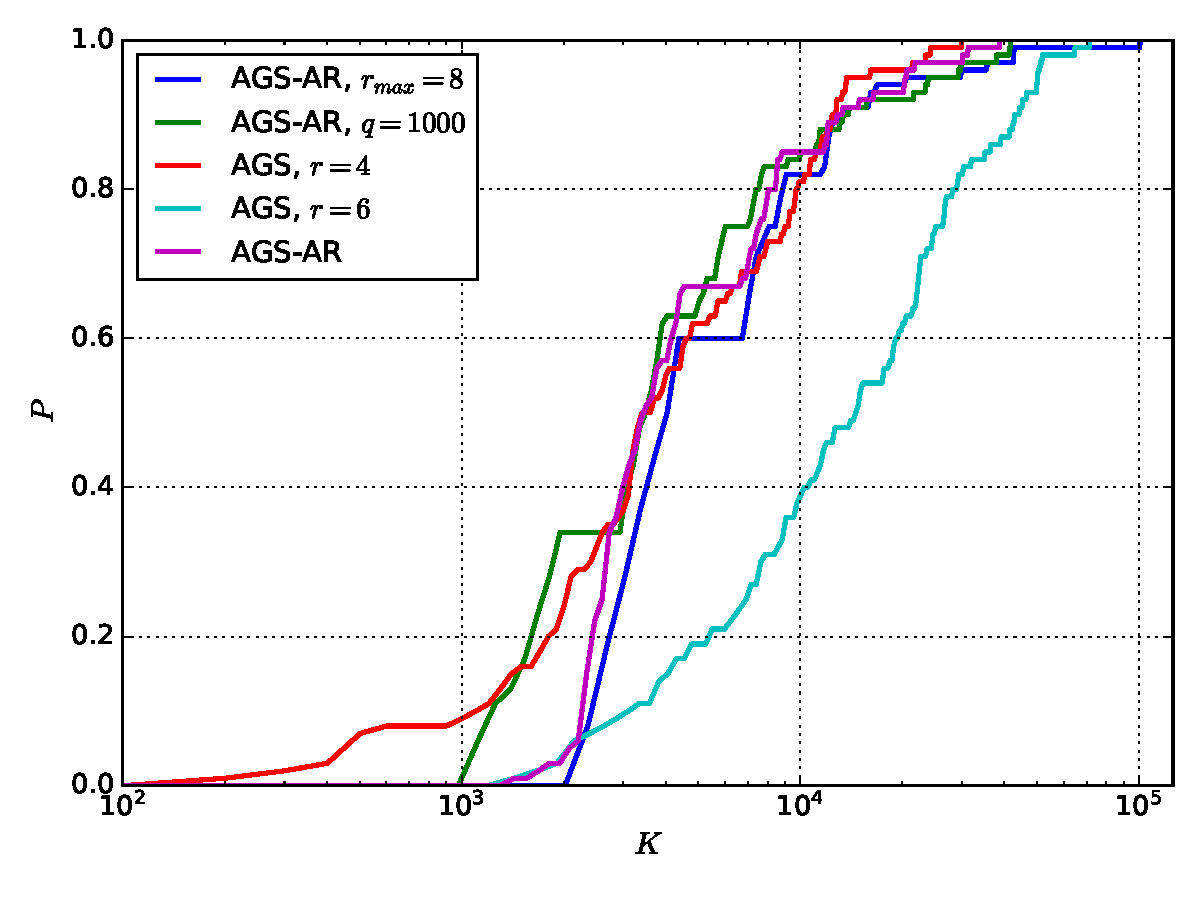
\includegraphics[width=.6\textwidth]{images/ar_stab.pdf}
  \caption{Operating characteristics of AGS and AGS-AR with different hyperparameters
  when solving problems from the GKLS 5d Simple classe. Best viewed in color.}
  \label{fig:stability}
\end{figure}

The operating characteristics collected in the experiments described above are shown in the Figure \ref{fig:stability}.
AGS with $r=6$ (the cyan-colored curve) shows the worst convergence speed, which indicates that AGS is very sensitive to choice of $r$.
Since on the start AGS-AR has the same value of $r$ as AGS with $r=6$, operating characteristics of these methods
are identical up to $K=2500$. After that point AGS-AR switches to $r=3$ and rapidly begins to increase the amount of solved problems
until the next exploration phase on $K=5000$. Intervals where AGS-AR works with $r=r_{max}$ are visible on the operating characteristics as plateaus.
Variations of $r$ and $q$ didn't drastically change the operating characteristic of AGS-AR. The latter observation shows robustness of the proposed
AGS modification with the alternating parameter $r$.

\section{Conclusions}

In the present paper, several global optimization algorithms were considered.
A comparison of efficiencies of these ones has been done on a set of test problems.
Also a scheme of hyperparameters control for the AGS algorithms was proposed and evaluated.
The results presented in this work allow making the following conclusions:
\begin{itemize}
  \item the proposed modification of the stock AGS, AGS-AR allows to pay less attention to initial hyperparameter tuning and
  performs on-par with properly tuned AGS;
  \item AGS-AR method has demonstrated the convergence
  speed and reliability at the level of DIRECT and exceeds many other algorithms, the open-source
  implementations of which are available;
  \item the stochastic optimization methods inferior to the deterministic ones in the convergence
speed and in reliability. It is manifested especially strongly on more complex multiextremal
problems.
\end{itemize}

\section{Алгоритм, решающий множество задач}

The feasible domain can also be defined by the constraints that essentially complicate the problem.
The problem statement in this case will take the following form:
\begin{equation}
  \label{eq:constrained_problem}
  \varphi(y^*)=\min\{\varphi(y):y\in G\},\:G=D \cap \{y: g_j(y)\leqslant 0, 1\leqslant j\leqslant m\}.
\end{equation}

Let us set \(g_{m+1}(y)=\varphi(y)\). Hereafter, we shall assume all functions
\(g_k(y),1\leqslant k \leqslant m+1\),
to satisfy the Lipschitz condition on the hyperinterval \(D\).


Further, let us consider solving a series of \(q\) problems of the kind
(\ref{eq:constrained_problem}):
\begin{equation}
  \label{eq:many_problems}
  \min\left\{\varphi_1(y), y\in G_1 \right\}, \min\left\{\varphi_2(y), y\in G_2\right\},...,
\min\left\{\varphi_q(y), y\in G_q\right\}.
\end{equation}

Далее следуя подходу, описанному в \cite{BarkalovStrongin2018}, для решения серии задач (\ref{eq:many_problems}) будем
использовать \(q\) синхронно работающих копий ИАГП с тем лишь отличием, что на шаге 6 при выборе
интервала с наилучшей характеристикой, выбор будет осуществляться из всех интервалов, которые
породили на данный момент \(q\) копий ИАГП. Если наибольшая характеристика соответствует
задаче \(i\), то выполняется шаг 7 в копии метода с номером \(i\), а остальные копии метода простаивают.
Таким образом, на каждой итерации испытание проводится в задаче, наиболее перспективной с точки зрения
характеристик (\ref{step3_1}), что позволяет динамически распределять ресурсы метода между задачами.

В \cite{BarkalovStrongin2018} приведена теория сходимости такого подхода на случай решения задач без ограничений.
При наличии ограничений характеристики интервалов, на концах которых нарушено разное количество ограничений,
вычисляются в соответствии с нижними строчками из (\ref{step3_1}). Нетрудно заметить, что и в этом случае
величины характеристик нормированы, а в случае точных оценок \(z_{\nu }^{*}\) и \(\mu _{\nu }\) их
масштаб не зависит от целевой функции и ограничений конкретной задачи. Таким образом, рассуждения
из \cite{BarkalovStrongin2018} можно провести и в случае использования индексной схемы.

Параллельная модификация метода не отличается от рассматриваемой в \cite{BarkalovStrongin2018}
и заключается в выборе \(p\) интервалов на шаге 6 и выполнения \(p\) испытаний параллельно
на следующем шаге. При этом все ресурсы метода в рамках итерации могут быть направлены как на одну, так и
на \(l\leqslant p\) задач одновременно (в зависимости от того, какой из задач принадлежат выбранные методам интервалы).

\subsection{Условия сходимости}
\label{sec:conv_method}

Достаточные условия сходимости иетода из Секции~\ref{sec:method} в случае \(q=1\) приведены в \cite{Strongin2000}.
\begin{theorem} (Достаточные условия сходимости AGS)
  \label{th:single_conv}
  Пердположим, что следующие утверждения справедливы:
  \begin{enumerate}
    \item \(D\ne\emptyset\), задача (\ref{eq:constrained_problem}) имеет решение.
    \item Функции \(g_j(y)\leqslant 0, 1\leqslant j\leqslant m + 1\), липшицевы в области \(D\) с соответствующими константами \(L_i\)
     (здесь \(g_{m+1}(y)=\varphi(y)\)).
    \item Для достаточно больших \(k\) из (\ref{eq:points}),
    значения \(\mu_\nu\) из (\ref{step2}) удовлетворяют неравенствам:
    \begin{equation}
      r_\nu\mu_\nu > 2^{3-1/N}L_\nu \sqrt{N+3},\: 1\leqslant \nu \leqslant m + 1.
    \end{equation}
  \end{enumerate}
  Тогда любая предельная точка \(\overline{y}\) последовательности \(\{y_k\} = \{y(x_k)\}\), сгенерированная
  AGS при решении задачи (\ref{eq:constrained_problem}) является допустимой и удовлетворяет условиям
\begin{equation}
  \label{eq:conv_cond}
  \varphi(\overline{y})=\inf\{ \varphi(y^k): g_i(y^k)\leqslant 0,1\leqslant i\leqslant m, k=1,2,\dots\}=\varphi(y^*).
\end{equation}
\end{theorem}

\begin{remark}
  \label{rem:r1}
  Из соотношения между константами Гёльдера и Липшица из неравенства (\ref{eq:conv_cond}) следует, что
  параметр \(r_\nu\) из (\ref{step3_1}) должен удовлетворять условию
  \begin{equation}
    r_\nu > 2^{2 - 1/N}.
  \end{equation}
\end{remark}

\begin{theorem} (О сходимости MIAGS) Пусть условия 1-3 Теоремы~\ref{th:single_conv} верны для каждой задачи \(i,\:1\leqslant i\leqslant q\) из (\ref{eq:many_problems}),
т.е. каждая из задач может быть решена AGS.
  Тогда в процессе решения \(q\) задач MIAGS сгенерирует
  \(q\) бесконечных последовательностей \(\{y^k_i\},\:1\leqslant i\leqslant q\), таких, что
  \begin{displaymath}
    \varphi_i(\overline{y_i})=\inf\{ \varphi(y^k_i): g^i_j(y^k_i)\leqslant 0,1\leqslant j\leqslant m_i, k=1,2,\dots\}=\varphi_i(y^*_i).
  \end{displaymath}
\end{theorem}
\begin{proof}
  Рассмотрим две случайно выбранные задачи из множества (\ref{eq:many_problems})
  \begin{equation}
      \begin{array}{lr}
        \min\{\varphi(y):y\in D_1,\: g_j^\varphi(y)\leqslant 0, 1\leqslant j\leqslant m_1\}, \\
        \min\{\psi(y):y\in D_2,\: g_j^\psi(y)\leqslant 0, 1\leqslant j\leqslant m_2\}.
      \end{array}
  \end{equation}
  Обозначим характеристики интервалов (\ref{step3_1}) в первой задаче как \(R_\varphi(i)\)
  и во второй задаче как \(R_\psi(j)\). Принимая во внимание обозначения, имеем:
  \begin{equation}
      \begin{array}{lr}
        R_\varphi(t_\varphi)=\max_{1\leqslant i\leqslant k}R_\varphi(i), \\
        R_\psi(t_\psi)=\max_{1\leqslant j\leqslant s}R_\psi(j),
      \end{array}
  \end{equation}
  где \(k\) обозначает количество испытаний, сделанных при решении первой задачи, а \(s\)
  это количество испытаний, сделанных при решении второй. Последовательность точек испытаний
  в первой задаче обозначим \(\{v^k\}\), во второй задаче \(\{u^s\}\).
  Значения \(z^k=g^\varphi_\nu(v_k),\nu =\nu (v_{k})\) соответствуют точкам \(\{v^k\}\),
  а значения \(w^s=g^\psi_\nu(u_s),\nu =\nu(u_{s})\) соответствуют точкам \(\{u^s\}\).

  Когда две задачи решаются одновременно, метод выбирает интервал для следубщего испытаний в
  соответствии с условием:
  \begin{equation}
    R(t) = \max\{R_\varphi(i),R_\psi(j)\}.
  \end{equation}

  Пусть алгоритм решает две задачи и счётчик испытаний равен \(l = k + s, l=0,1,2,\dots\).
  Тогда, поскольку Теорема~\ref{th:single_conv} справедлива для обеих задач, как минимум одна из последовательностей
  \(\{v^k\}\) или \(\{u^s\}\) будет бесконечной (пусть это \(\{v^k\}\)).
  Если доказать, что обе последовательности бесконечны, то это будет означать наличие сходимости в обеих задачах.

  Рассмотрим предельную точку \(\overline{v}\in [v_{i-1},v_i]\), где \(i=i(k)\). Индексы \(v_{i-1}\;,v_i\)
  могут быть равны или различаться, но в силу сходимости, при достаточно больших \(k\) будут стабильны.
  %will be steady  equal to \(m_1+1\) (if \(\overline{v}\) is
  %an interior point of the feasible domain produced by constraints \(g^\varphi_p(y),p=\overline{1,m_1}\))
  %or \(\nu(v_{i-1})\ne\nu(v_i)\) (if \(\exists p: 1\leqslant p\leqslant m_1, g^\varphi_p(y(\overline{v}))=0\)).
  В первом случае алгоритм будет испльзовать первую ветку правила (\ref{step3_1}), иначе он будет применять одну из оставшихся ветвей.

  Рассмотрим сначала первый случай: из (\ref{step2})
  \begin{displaymath}
    \frac{|z_i-z_{i-1}|}{\Delta_i} \leqslant \mu_{\varphi,\nu}.
  \end{displaymath}
  Принимая во внимание это неравенстов, получим верхнюю оценку:
  \begin{displaymath}
    \frac{(z_i-z_{i-1})^2}{r_\nu^2\mu_{\varphi,\nu}^2\Delta_i}=\frac{(z_i-z_{i-1})^2\Delta_i}{(r_\nu\mu_{\varphi,\nu}\Delta_i)^2}
    \leqslant \frac{\Delta_i}{r_\nu^2}.
  \end{displaymath}
  Таким образом, при использовании первой ветки правила (\ref{step3_1}) справедливо неравенство
  \begin{equation}
    \label{eq:th1}
    R_\varphi(i)\leqslant\Delta_i(1 + \frac{1}{r_\nu^2}) - \frac{2(z_i+z_{i-1}-2z^*_\nu)}{r_\nu\mu_{\varphi,\nu}}.
  \end{equation}
  Поскольку \(\overline{v}\) является предельной точкой последовательности \(\{v^k\}\) и \(\varphi(y(\overline{v}))\leqslant z^*_{\nu}, \nu=m+1\) или
  \(z^*_\nu=0, \nu<m+1\) и \(z_{i-1},z_i\to 0\) при \(k\to\infty\):
  \begin{equation}
    \label{eq:th2}
    \Delta_i\to 0, z_i+z_{i-1} - 2 z_\nu^*\to 0.
  \end{equation}
  Во втором случае (когда применяется одна из оставшихся ветвей правила (\ref{step3_1})) имеем:
  \begin{displaymath}
    R_\varphi(i)=2\Delta_i - 4\frac{z_i-z^*_\nu}{r_\nu\mu_{\varphi,\nu}}.
  \end{displaymath}
  Если \(z^*_\nu \ne 0\), то \(z_i-z^*_\nu \geqslant 0\) и
  \begin{equation}
    \label{eq:th3}
    R_\varphi(i)=2\Delta_i - 4\frac{z_i-z^*_\nu}{r_\nu\mu_{\varphi,\nu}} \leqslant 2\Delta_i.
  \end{equation}
  Иначе, поскольку \(\overline{v}\) это допустимая точка, \(z_i\to 0\) при \(k\to\infty\).

  Из (\ref{eq:th1}) (\ref{eq:th2}) (\ref{eq:th3}) для любого маленького \(\delta > 0\) существует достаточно большое значение \(k\) такое, что
  \begin{equation}
    R_\varphi(i)\leqslant \delta.
    \label{eq:th6}
  \end{equation}

  Пусть \(\alpha = \max\{\nu(u):u\in\{u^s\}\}\). Т.к. \(\alpha\) это текущий максимальный индекс
  в поисковой последовательности \(\{u^s\}\), то в соответствии с правилом (\(\ref{eq:step_4}\)), \(\exists j: w^*_\alpha=w_j\).

  Если \(\nu(w_{j-1})=\nu(w_{j})=\alpha\), то применяется первая ветка правила (\ref{step3_1}) и
  \begin{equation}
    \begin{array}{l}
      R_\psi(j)=\Delta_j + \frac{(w_j-w_{j-1})^2}{r_\alpha^2\mu_{\psi,\alpha}^2\Delta_j}
        - \frac{2(w_j+w_{j-1}-2w^*_\alpha)}{r_\alpha\mu_{\psi,\alpha}} \geqslant \\
        \geqslant\Delta_j - \frac{2(w_j+w_{j-1}-2w^*_\alpha)}{r_\alpha\mu_{\psi,\alpha}} =
        \Delta_j - \frac{2\Delta_j(w_{j-1}-w_j)}{r_\alpha\mu_{\psi,\alpha}\Delta_j} \geqslant\\
        \geqslant \Delta_j - \frac{2\Delta_j}{r_\alpha} = \Delta_j\left(1-\frac{2}{r_\alpha}\right).
      \end{array}
    \label{eq:th4}
  \end{equation}

  Если \(\nu(w_{j-1})\ne\nu(w_{j})=\alpha\), то \(\nu(w_{j-1})<\alpha\) и применяется третья ветка правила (\ref{step3_1}):
  \begin{equation}
    R_\psi(j)=2\Delta_j - 4 \frac{w_j-w^*_{\alpha}}{r_\alpha \mu_{\psi,\alpha}}=2\Delta_j > 0.
    \label{eq:th5}
  \end{equation}
  Принимая во внимание Зачечание~\ref{rem:r1}, (\ref{eq:th4}), (\ref{eq:th5}), можно сделать вывод о том, что
  существует интервал с положительной характеристикой характеристикой \(R_\psi(j)>0\). В то же время, выполняется (\ref{eq:th6})
  и неравенство
  \begin{displaymath}
    R_\psi(j) > R_\varphi(i)
  \end{displaymath}
  будет справедливым при достаточно большом \(k\). Таким образом, следующее испытание будет совершено
  в интервале, соответствующему второй задаче с целевой функцией \(\psi(y)\), и последовательность \(\{v^s\}\) будет бесконечной.

  Поскольку были рассмотрены две произвольные задачи из \(q\) задач, теорема верна для любой пары задач рассматриваемого множества.
  По индукции, теорема также верна и для всего множества.
\qed
\end{proof}


\section{Результаты численных экспериментов}

Использование сгенерированных некоторыми случайными механизмами
наборов тестовых задач с известными решениями является одним из общепринятых подходов
к сравнению алгоритмов оптимизации \cite{Beiranvand2017}. В данной работе
будем использовать два генератора тестовых задач, порождающих задачи различной природы \cite{grishaginClass, Gaviano2003}.
Эти генераторы порождают задачи без нелинейных ограничений, поэтому в дополнение к ним использована
система GCGen \footnote{Исходный код системы доступен по ссылке https://github.com/UNN-ITMM-Software/GCGen} \cite{GergelBarkalov2019}, позволяющая генерировать задачи с ограничениями на основе произвольных нелинейных
функций.

Вместе с системой GCGen распространяются примеры ее использования и построения
наборов задач, каждая из которых состоит из целевой функции и двух ограничений,
порожденных генератором \(F_{GR}\) \cite{grishaginClass} или GKLS \cite{Gaviano2003}.

% Обозначим набор из 50 задач, полученных с помощью GCGen и первого генератора из \cite{grishaginClass} как \(F_{GR}^C\). Механизм построения функций \(F_{GR}\) не предусматривает контроля за размерностью (она равна 2) и количеством локальных оптимумов, однако известно, что порождаемые функции
% являются существенно многоэкстремальными.

Генератор GKLS \cite{Gaviano2003} позволяет получать функции заданной размерности и с заданным количеством экстремумов.
В сочетании с GCGen были порождены два множества по 100 задач размерности 2 и 3. Каждая из задач имеет два ограничения.
Также с целью демонстрации того, что свойства метода сохраняются при существенно разных свойствах задач
был сгенерирован смешанный класс, состоящий из 50 задач с двухмерными функциями GKLS и 50 задач с функциями \(F_{GR}\).
На рис. \ref{fig:isolines} представлены примеры линий уровня рассматриваемых задач. Допустимая область закрашена.

\begin{figure}[ht]
    \centering
    \subfloat[Решение внутри допустимой области]{
    {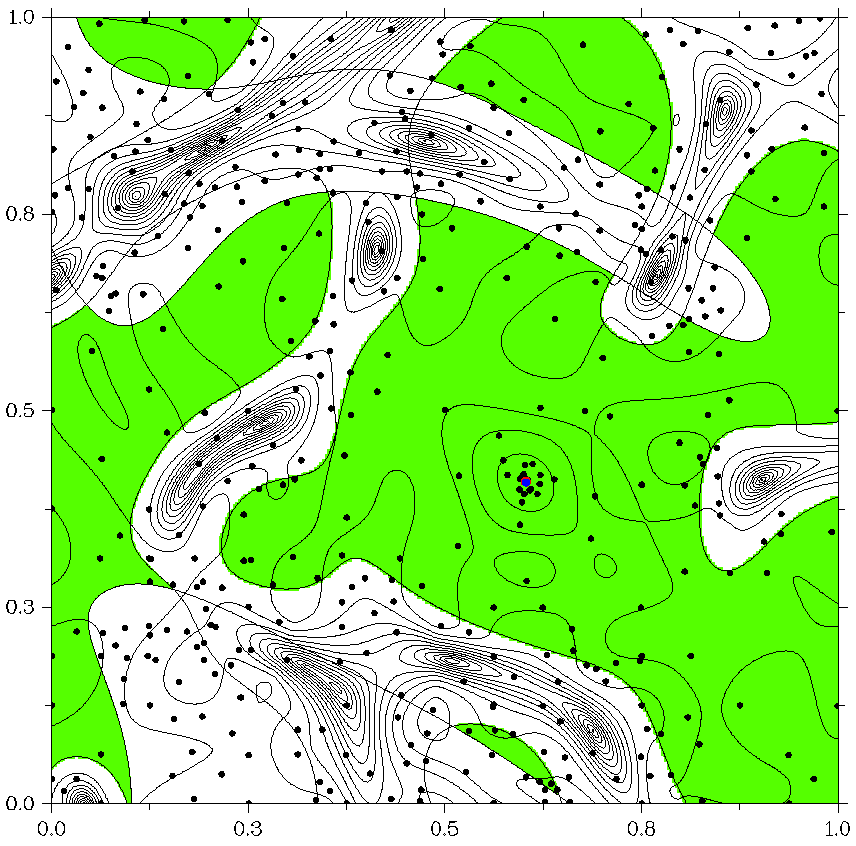
\includegraphics[width=.5\textwidth]{images/2.png}}}
    \subfloat[Решение на границе допустимой области]{
    {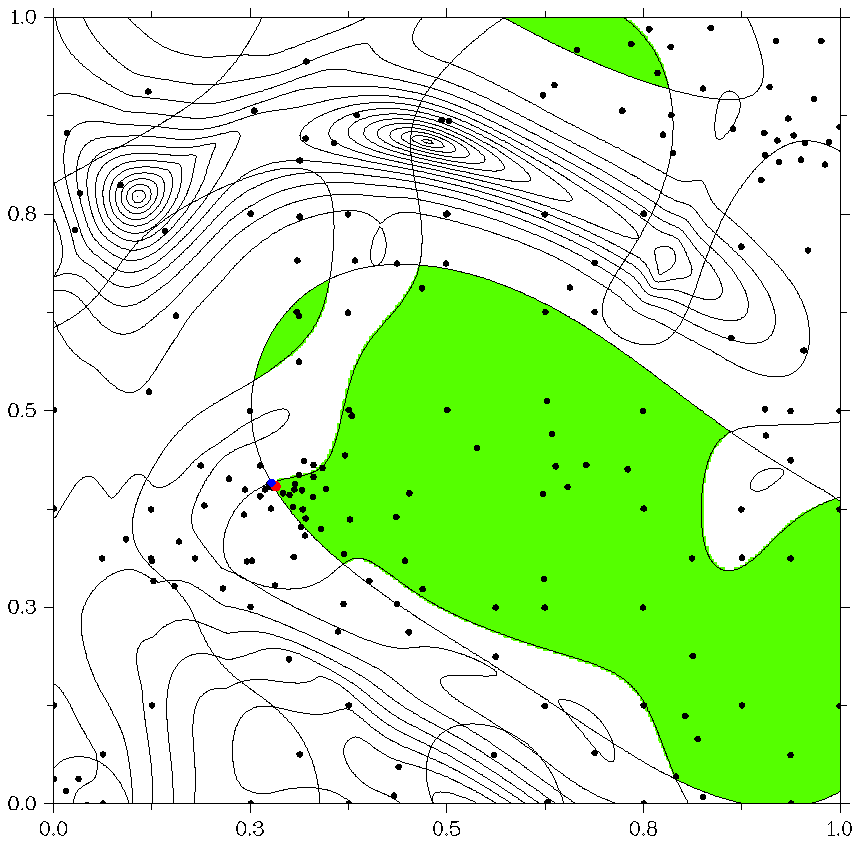
\includegraphics[width=.5\textwidth]{images/4.png}}}
    \caption{Линии уровня и точки испытаний ИАГП в двух синтетических задачах}
    \label{fig:isolines}
\end{figure}

Будем считать, что тестовая задача решена, если метод оптимизации провел очередное испытание \(y^k\) в
\(\delta\)-окрестности глобального минимума \(y^*\), т.е. $\left\|y^k-
y^*\right\|\leqslant \delta = 0.01\left\|b-a\right\|$, где \(a\) и \(b\) --- левая и правая границы гиперкуба из (\ref{eq:task}).
Если указанное соотношение не выполнено до истечения лимита на количество испытаний, то задача считается нерешенной.

%В качестве характеристик метода оптимизации на каждом из классов будем рассматривать среднее число
%испытаний, затраченное для решения одной задачи, и количество решенных задач. Чем меньше число испытаний, тем быстрее метод сходится
%к решению, а значит и меньше обращается к потенциально трудоемкой процедуре вычислений целевой функции.
При оценке качества метода и его реализации кроме ускорения от распараллеливания и времени выполнения также будем принимать во внимание среднее максимальное расстояния (в смысле \(l_{\inf}\)-нормы) текущей оценки оптимума до его реального положения,
вычисленное на множестве задач (\ref{eq:many_problems}): \(D_{avg}\) и \(D_{max}\). Динамика этих величин в процессе оптимизации
показывает, насколько равномерно метод распределяет ресурсы между задачами.

Реализация параллельного метода была выполнена на языке C++ с использованием технологии OpenMP
для распареллеливания процесса проведения испытаний на общей памяти. Все вычислительные
эксперименты проведены на машине со следующей конфигурацией: Intel Core i7-7800X, 64GB RAM, Unubtu 16.04 ОS, GCC 5.5 compiler.

\subsection{Результаты решения сгенерированных задач}

Результаты решения тестовых задач последовательной и параллельной версией модифицированного ИАГП
для решения множества задач представлены в таблице \ref{tab:speedup}. Для всех двухмерных классов задач параметр \(r=4.7\).
В случае трехмерных задач \(r=4.7,\: \varepsilon_\nu=0.1\).
Во всех экспериментах в целевые функции и ограничения была внесена дополнительная вычислительная нагрузка так,
чтобы время одного обращения к функции задачи было равно примерно 1мс.

Из таблицы видно, что ускорение по итерациям \(S_i\) растет линейно с увеличением числа потоков \(p\),
в то время, как ускорение по времени \(S_p\) увеличивается не так быстро, что говорит о неидеальной
реализации алгоритма. Увеличить реальное ускорение, верхней границей для которого является
\(S_i\), возможно путем оптимизации взаимодействий между копиями ИАГП и это планируется сделать в ходе будущей работы.

\begin{table}
  \centering
  \caption{Результаты экспериментов на наборах синтетических задач}
  \label{tab:speedup}
  \begin{tabular}{c|c|cccc}
    %\cline{1-8}\noalign{\smallskip}
    Класс задач & \textit{p} & Количество итераций & Время, с & \(S_i\) & \(S_t\)   \\
    %s\noalign{\smallskip} \cline{4-5} \cline{7-8}  \noalign{\smallskip}
    \hline
    GKLS \& \(F_{GR}\) based \
      & 1 & 51434 & 90.20 & -    & - \\
      & 2 & 25698 & 56.96 & 2.00 & 1.58 \\
      & 4 & 13015 & 36.67 & 3.95 & 2.46 \\
      & 6 & 8332  & 26.85 & 6.17 & 3.36 \\
    \hline
    GKLS based 2d \
      & 1 & 59066 & 97.53 & -    & - \\
      & 2 & 29060 & 60.56 & 2.04 & 1.61 \\
      & 4 & 14266 & 38.92 & 4.14 & 2.51 \\
      & 6 & 9436  & 29.53 & 6.26 & 3.30 \\
    \hline
    GKLS based 3d \
      & 1 & 782544 & 1117.55 & -    & - \\
      & 2 & 397565 & 752.92  & 1.97 & 1.48 \\
      & 4 & 208073 & 526.67  & 3.76 & 2.12 \\
      & 6 & 142089 & 445.45  & 5.50 & 2.51 \\
    \hline
  \end{tabular}
\end{table}

Для того, чтобы показать равномерную сходимость все тестовые задачи были также решены ИАГП
в режиме решения отдельных задач. На рис. \ref{fig:devs_mixed} указаны графики величин
средних и максимальных расстояний от реальных оптимумов до их текущих оценок при решении
серии из задач, порожденных двумя разными генераторами, по отдельности (сплошная кривая) и совместно (пунктирная кривая).
Не смотря на значительную разницу в структуре задач, модифицированный ИАГП
гораздо быстрее уменьшает как максимальное, так и среднее отклонение оценок от оптимумов.
Это говорит о наличии равномерной сходимости по всему множеству совместно решаемых задач.
При этом в случае последовательного решения задач величина \(D_{max}\) имеет наибольшее значение вплоть
до решения последней задачи.

\begin{figure}[ht]
    \centering
    \subfloat[\(D_{max}\)]{
    \label{fig:max_dev} {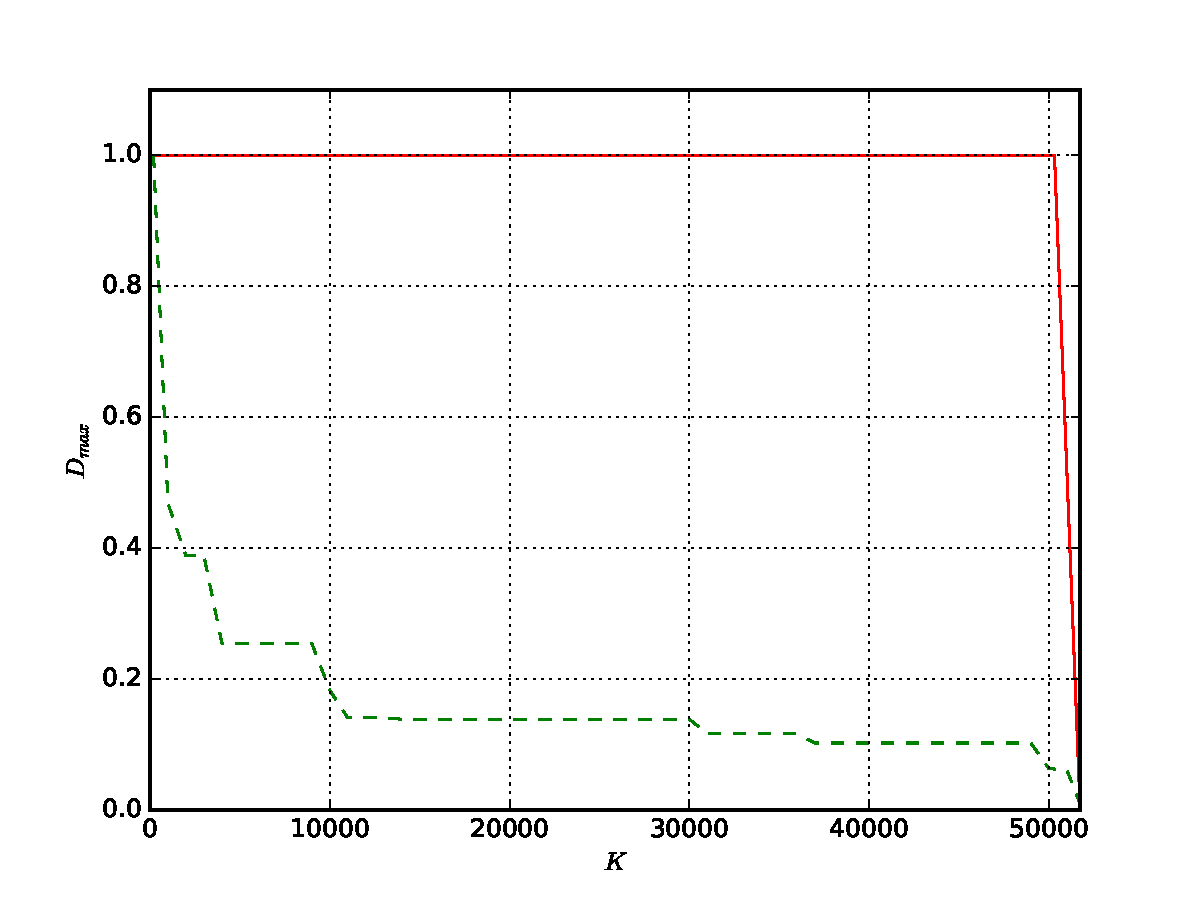
\includegraphics[width=.5\textwidth]{images/mixed_2d_max.pdf}}}
    \subfloat[\(D_{avg}\)]{
    \label{fig:avg_dev} {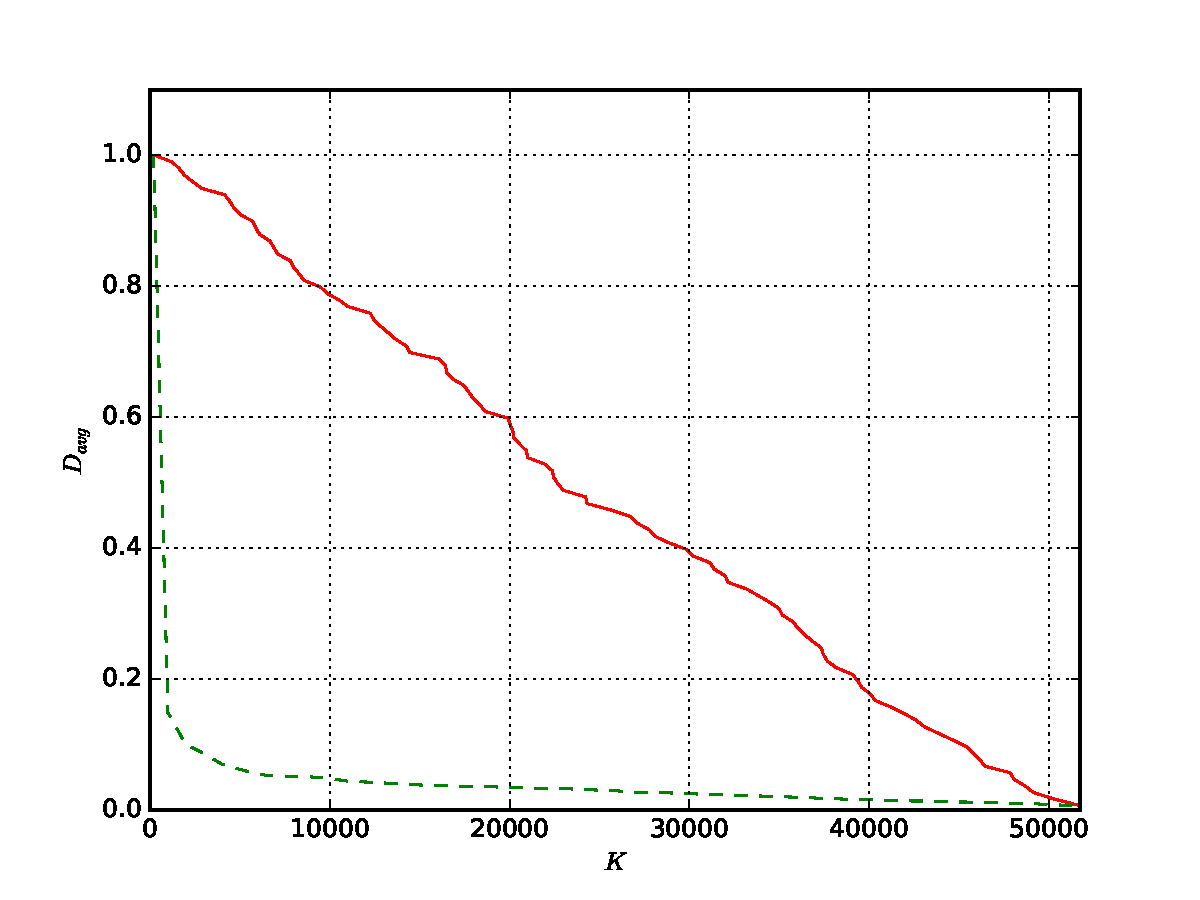
\includegraphics[width=.5\textwidth]{images/mixed_2d_avg.pdf}}}
    \caption{Динамика величин \(D_{avg}\) и \(D_{max}\) в процессе решения множества двухмерных задач,
    порождённых двумя разными генераторами GKLS и \(F_{GR}\)}
    \label{fig:devs_mixed}
\end{figure}

\subsection{Пример решения многокритериальной задачи}

Для демонстрации эффективности подхода к балансировке нагрузки рассмотрим пример,
в котором множество задач вида (\ref{eq:many_problems}) порождено в результате скаляризации
многокритериальной задачи оптимизации с ограничениями.

Рассмотрим тестовую задачу, предложенную в \cite{BinhKorn1999}:
\begin{equation}
  \label{eq:mco_probem}
  \begin{array}{l}
      Minimize \left \{
      \begin{array}{l}
        f_1(y) = 4 y_1^2 + 4 y_2^2 \\
        f_2(y) = (y_1-5)^2 + (y_2-5)^2 \\
      \end{array}
      \right .
      y_1\in [-1;2],y_2\in [-2;1]
      \\s.t.
      \\
      \left \{
      \begin{array}{l}
        g_1(y) = (y_1 - 5)^2 + y_2^2 - 25 \leqslant 0 \\
        g_2(y) = -(y_1 - 8)^2 - (y_2 + 3)^2 + 7.7 \leqslant 0\\
      \end{array}
      \right .
  \end{array}
\end{equation}

Будем использовать свертку Гермейера для скаляризации задачи (\ref{eq:mco_probem}).
После свертки скалярная целевая функция имеет вид:
\begin{equation}
  \varphi(y,\lambda_1,\lambda_2)=\max\{\lambda_1 f_1(y), \lambda_2 f_2(y)\},
\end{equation}
где \(\lambda_1,\lambda_2\in[0,1],\: \lambda_1+\lambda_2=1\). Перебирая все возможные
коэффициенты свертки, можно найти все множество парето-оптимальных решений в
задаче (\ref{eq:mco_probem}). Для численного построения множества Парето выберем
100 наборов коэффициентов \((\lambda_1,\lambda_2)\) таких, что
\(\lambda_1^i=i h,\: \lambda_2^i=1-\lambda_1^i,\: h=10^{-2},i=\overline{1, 100}\).

В качестве ограничения на вычислительные ресурсы был выбран лимит в 2500 испытаний.
Множество вспомогательных скалярных задач решалось двумя способами:
\begin{itemize}
  \item каждая задача решается отдельно с помощью ИАГП с установленным лимитом в
  25 испытаний. Таким образом, вычислительные ресурсы равномерно распределены между задачами;
  \item все задачи решаются одновременно с помощью обобщенного ИАГП с установленным лимитом в
  2500 испытаний.
\end{itemize}
В обоих случаях параметр \(r=4\).

\begin{figure}[ht]
    \centering
    \subfloat[ИАГП, раздельное решение задач]{
    \label{fig:mco_pareto_1} {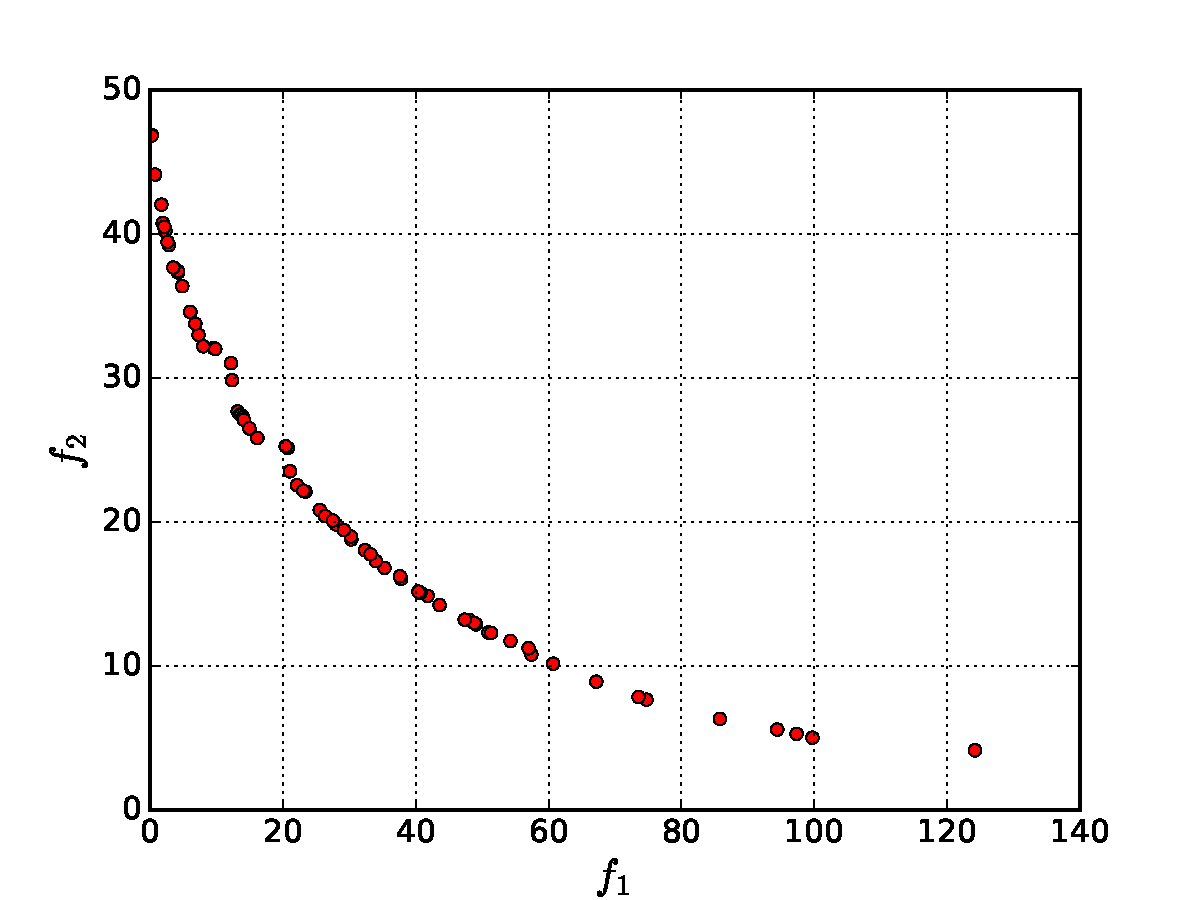
\includegraphics[width=.5\textwidth]{images/single_mco.pdf}}}
    \subfloat[ИАГП для множества задач]{
    \label{fig:mco_pareto_2} {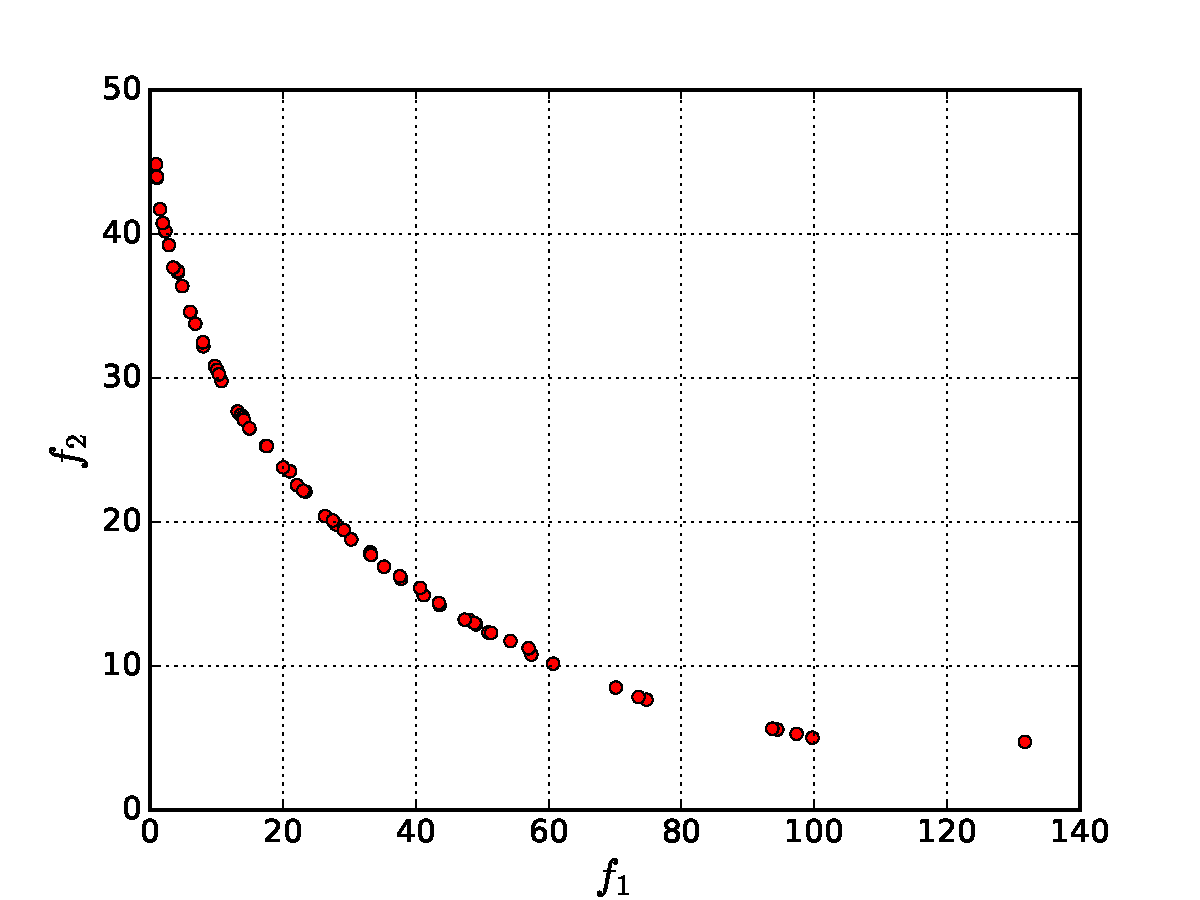
\includegraphics[width=.5\textwidth]{images/multi_mco.pdf}}}
    \caption{Численные оценки множества Парето в задаче (\ref{eq:mco_probem}), полученные после 2500 испытаний}
    \label{fig:mco_pareto}
\end{figure}

На рис. \ref{fig:mco_pareto} представлены графики решений, полученных каждым из методов.
Все графики качественно совпадают с указанным в \cite{BinhKorn1999} (авторы не предоставили другой
информации и решениях для сравнения). Видно, что на рис. \ref{fig:mco_pareto_1}
кривая Парето имеет вогнутости, что не соответствует решению, указанному в \cite{BinhKorn1999} и
означает нехватку ресурсов для решения некоторых из вспомогательных задач.
Для оценки качества решения также был вычислен показатель \(Spacing(SP)\) \cite{RiquelmeLucken2015},
характеризующий плотность точек аппроксимации множества Парето.
\begin{displaymath}
  SP(S)=\sqrt{\frac{1}{|S|-1} \sum_{i=1}^{|S|} (\overline{d}-d_i)^2},
  \:\overline{d}=mean\{d_i\},\:d_i=\min_{s_i,s_j\in S:s_i\ne s_j}||F(s_i)-F(s_j)||_1,\: F=(f_1,f_2)
\end{displaymath}
В случае отдельного решения задач \(SP_{single}=0.984\), а при решении задач методом с балансировкой нагрузки
\(SP_{multi}=0.749\), что говорит о более качественном приближении решения.

\section{Заключение}

В ходе практической работы была реализована поддержка нелинейных ограничений в алгоритме, решающeм
множество задач глобальной оптимизации. Проведены численные эксперименты, демонстрирующие
преимущество рассматриваемого подхода над решением задач по отдельности. Показана эффективность
совместного решения множества задач на примере решения многокритериальной задачи с
нелинейными ограничениями.

В ходе дальнейшей работы планируется улучшить текущую реализацию алгоритма,
сократив расходы на содержание поисковой информации для множества задач и тем самым улучшив
показатели параллельного ускорения по времени. Также планируется реализовать версию
рассматриваемого алгоритма, работающего на распределенной памяти по схеме, описанной в \cite{BarkalovLebedev2017_2}.

По результам практики было проведено выступление с устным докладом на конференции Параллельные вычислительные технологии (ПАВТ`2020).

\cs{Заключение}

В рамках квалификационной работы была поставлена цель выбрать оптимальную модификацию алгоритма глобального поиска (AGS)
и на его основе построить метод для одновременного решения множества задач глобальной оптимизации с нелинейными ограничениями.

В ходе работы получены следующие результаты:
\begin{enumerate}
    \item произведено сравнение различных способов редукции размерности, основанных на отображениях типа кривой Пеано.
    В результате был сделан вывод о том, что для построения базовой многомерной версии метода AGS 
    с практической стороны наиболее выгодно использовать единственную кривую Пеано;
    \item предложена модификация AGS, AGS-AR, менее чувствительная к параметрам, и сходящаяся так же быстро, как AGS
    с заранее подобранными под класс задач параметрами;
    \item AGS-AR продемонстрировал надёжность и скорость сходимости на уровне другого детерминированного метода, DIRECT,
    и превзошёл на рассмотренных тестовых задачах многие другие методы, реализации которых так же доступны в исходных кодах;
    \item программная реализация метода AGS-AR прошла процедуру ревью и была включена в состав популярной библиотеки
    алгоритмов нелинейной оптимизации NLOpt;
    \item реализована поддержка нелинейных ограничений в алгоритме, решающeм
    множество задач глобальной оптимизации в совокупности и распределяющего свои ресурсы так, чтобы
    обеспечивать равномерную сходимость во всех задачах. Доказано теорема о достаточных условиях сходимости
    полученного метода. Свойство равномерной сходимости проверено с помощью численного эксперимента.
\end{enumerate}


%\newpage
%\nocite{*}
\addcontentsline{toc}{section}{Список литературы}
\printbibliography

Подпись аспиранта \Repeat{25}{\_}
%\input{attachments}

\endgroup

\end{document}
